%\addcontentsline{toc}{chapter}{Development Process}
\chapter{Design}

This chapter mainly covers the design and processes by which a prototype was designed and implemented. The chapter goes into detail about the intended structure and implementation of the program and UI structure. A significant part of this project consisted of the UI, and its interactions, so much detailed effort is spent on explaining various design decisions and attempting to explain it all goes together into the programming portion of the project.

Firstly, a discussion about the prototype design (Section \ref{PROTOTYPESECTION}), then changes to that design as implementation occurred (Section \ref{DESIGNCHANGESSECTION}), then the code structure and how different parts of the application fit together (Section \ref{CODESTRUCTUREDESIGN}), and finally rounding it up with the design aspects based around accessibility (Section \ref{ACCESSIBILITYDESIGN}).


\section{User Interface Prototyping} \label {PROTOTYPESECTION}
A significant part of the design process in this project was user interface prototyping, it was the main focus of a sprint and was the most significant driving force behind the design of the entire application, so the time spent was justified. I found the process of prototyping to be incredibly valuable when it came to getting my head around what features would make sense, in the context of a native application, against what would not work in the sense of a Material Design based native Android application.

The prototype was created using a web app called Figma \cite{FIGMA}, and my version can be found at this URL \url{https://bit.ly/2xuAvl6}, from here you can see the entire prototype, as well as access a semi-functional version, not all functionality was implemented due to certain limitations with the prototyping software and time limitations. Still, it gives a good idea of how the application was designed and intended to run before any code was written.

\subsection{Colour Scheme} \label{COLOURSCHEME}
In order to stick to Material Design guidelines, I utilised a tool provided by the Material Design website\cite{MATERIALDESIGNCOLOURS} for determining what secondary and aspect colours should be used, given a set of primary colours, that are common across multiple applications. The idea of this colour tool is to promote the idea of applications on Android having similar colour schemes, and a generalised theme across the entire platform. Early on, I liked a darker orange colour as my primary colour (\#ff6f00), I found it looked good in my prototype, and I stuck to it. The colour tool recommended a lighter primary colour (\#ffa040), and a darker primary colour(\#c43e00) for different parts of the application, such as the application navigation bar at the bottom of the phone, or the background of the system bar at the top of the Android phone. The lighter primary colour is often used for accenting or less important parts of the application. With the colour scheme, the text colour of black (\#000000) is recommended.

More modern Android applications, take advantage of a recent trend in UX design, which is the replaceable theme, with a darker version, for night time or general use, these themes use less power and often are easier on the eyes especially in low light environments. With that in mind, with the help of the aforementioned tool for colour picking\cite{MATERIALDESIGNCOLOURS}, I picked a dark variation colour scheme, primary colour (\#424242), primary light colour (\#6d6d6d), primary dark colour (\#1b1b1b), and text colour (white: \#ffffff). The dark theme mostly consists of different variations of the colour grey. To continue the application's theme across both dark and light themes, different parts of the application won't change, such as the title bar's background colour, or the colour of the \gls{Bottom Navigation Bar}'s icons.

The text colour changes based on the background colour, allow users of all abilities to read it easier, for example, white text on a black background is easier to read than a dark blue text on a black background. The same could be said for black text on a white background such as this report if the text were a light yellow, it would be harder to read on this light background.

\subsection{General App Design}

The app design has a few key features shared across multiple screens; this section discusses these key features.

The \gls{Bottom Navigation Bar} is the Material Design inspired navigation method of choice on Android according to the Material Design guidelines (\cite{MATERIALDESIGNGUIDELINES}), the current choice of only allowing navigation to home, cat finder, and saved cats (See Figure \ref{fig:prototype_home}) allows the main actions that users probably want to fulfil, to be the most available to users the moment they open the app. The \gls{Bottom Navigation Bar} allows a user to easily switch between the main screens using only one hand as it is near the base of the phone, is one of the main benefits of it's intended inclusion.

When on one of the main screens (Home, Cat Finder, and Saved Cats), there is the option to access the navigation draw (Section \ref{PROTOTYPENAVIGATIONDRAW}) using the \gls{Hamburger Icon} in the upper left side, featured throughout other Android application designs. However, due to the nature of the app, there are multiple different methodologies for navigation. In Android, there is the \gls{System Bar} and in-app navigation. Material Design has a guideline for navigation draw and navigation, it aims to replace the navigation draw button with an \gls{Up Button}, whenever you are not on any of the main screens, this allows a user to navigate back up the navigation hierarchy in the application quickly, the replacement is done fluidly with an animation. 

If a user navigates to a \gls{Card} from the main screens or a secondary screen, it navigates to either the Adoption Information screen or the Cat Information screen, which allows navigation back using an X button to close the current "pop-up".

It is possible to access the settings from the majority of the app (by clicking the cog icon in the top right of most of the screens in the app). The design is aimed at allowing users to get to the settings as fast as possible from wherever in the app. Quick access to settings is good because of the need to change key settings that may be added in the future for accessibility features or notifications, or if a user just doesn't want to lose their place in the app.

Material design provides a set of icons, the idea of having a single set of defined icons that are supported across multiple devices, applications, and interfaces aim to increase usability, and ease of learning for these devices, applications, and interfaces. The icons are the same across different devices and applications, for example, a settings icon is a cog, or a save icon is the floppy disk. Not only are these icons provided freely under an open license, but they are heavily integrated into the Android Studio integrated development environment.

\subsection{Home Screen}

\begin{figure} [htbp!]
    \centering
    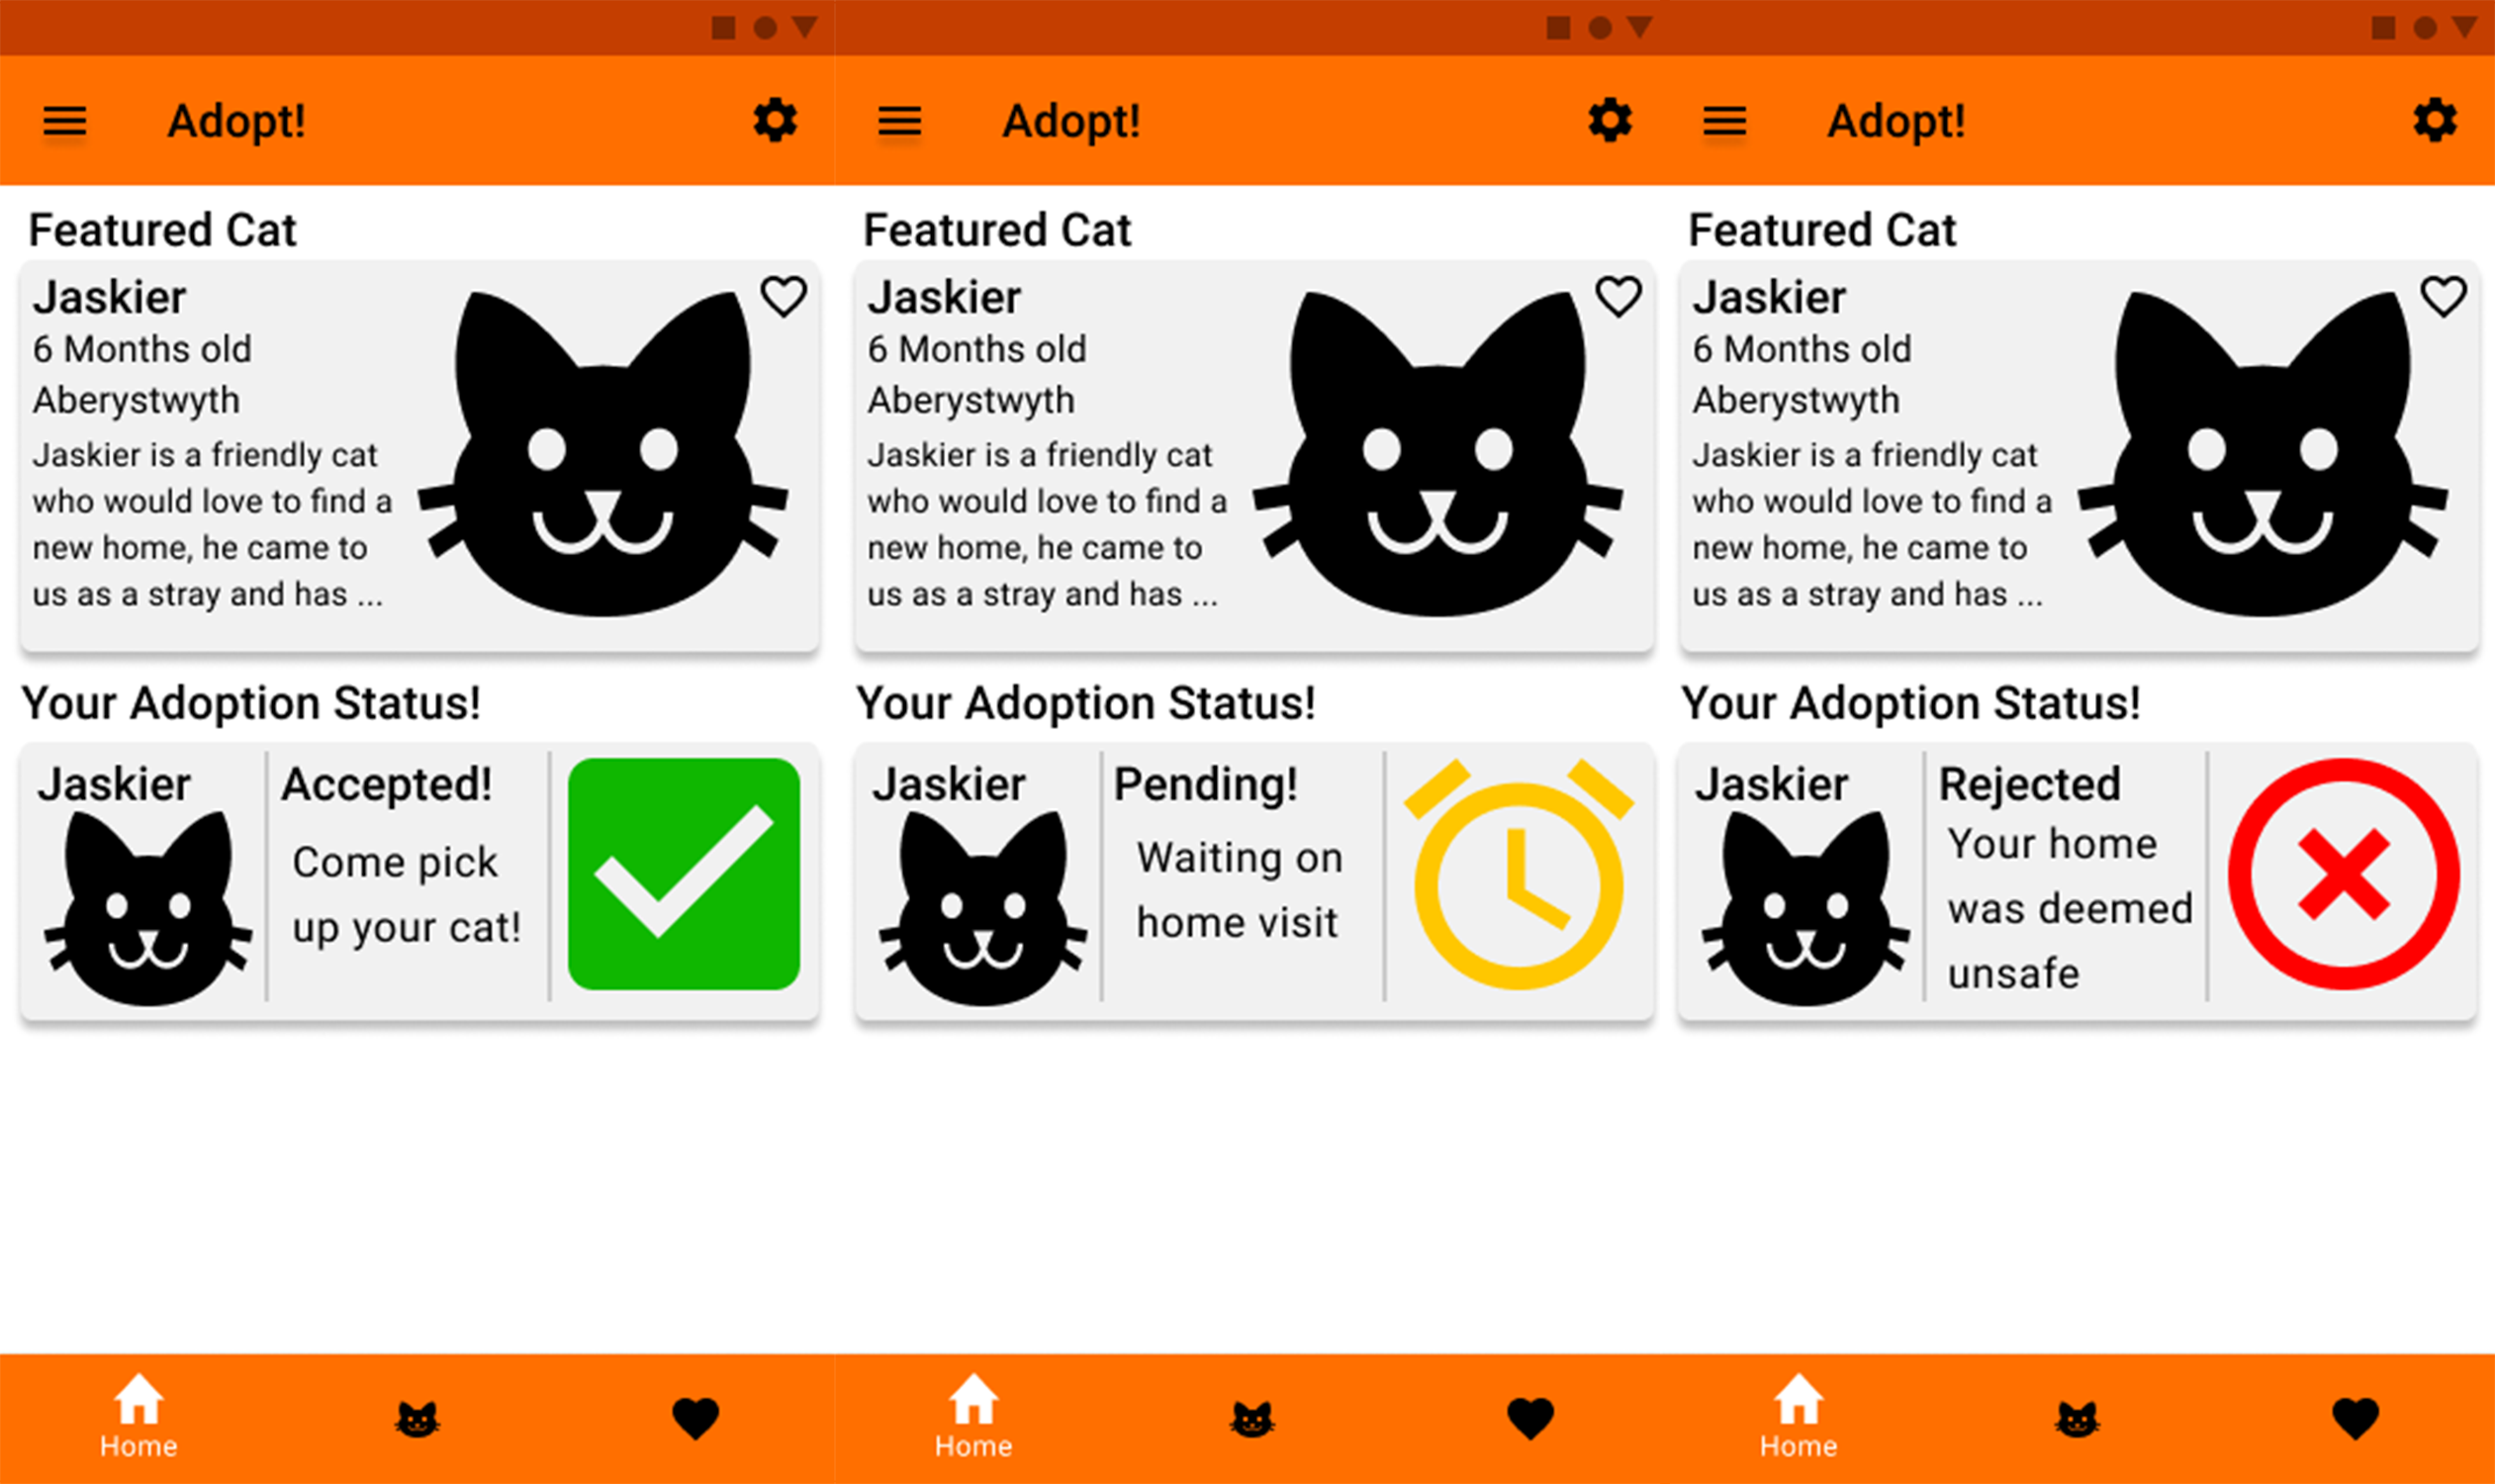
\includegraphics[height=7cm]{Images/PrototypeHomeScreen.png}
    \caption{3 variations of the prototyped home screen}
    \label{fig:prototype_home}
\end{figure}

Figure \ref{fig:prototype_home}, shows the prototype of my home page; it aims to have a randomly picked cat from the back end database showing using a Saved Cat Card (\ref{PROTOTYPESAVEDCATCARD}). On the home page, if logged in, it displays the statuses of your current adoption requests, figure \ref{fig:prototype_home} shows the adoption status cards (\ref{PROTOTYPEADOPTIONSTATUSCARD}) in it's 3 potential states, as there are multiple outcomes from a request if the user is not logged in, then text displays telling them there are not logged in and to login, to use that feature. My thought process with this layout was based around the idea of what people want to see the most, people want to see a cat to adopt, and most importantly users want to see their adoption status as soon as possible.

\subsection{Cat Finder Screen}

\begin{figure} [htbp!]
    \centering
    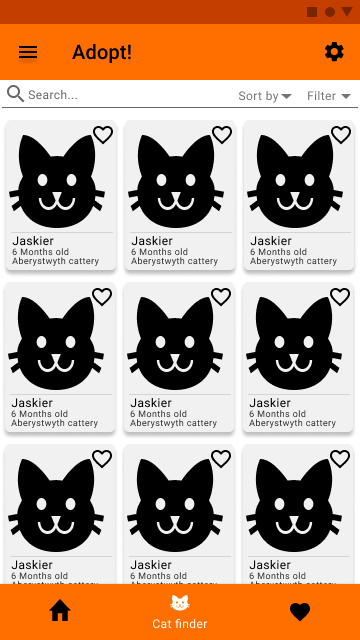
\includegraphics[height=7cm]{Images/PrototypeCatFinder.png}
    \caption{Prototype cat finder screen}
    \label{fig:prototype_cat_finder}
\end{figure}

The Cat finder screen is intended for users to find a cat to adopt, to allow for this it requires cats to be displayed similar to how Amazon or eBay lists products, as they are great inspirations for displaying options. In line with that, I included Search, Sort by and Filter functionality found in many e-commerce implementations, both on mobile and not, it has become a staple and expected feature of many places offering both products for sale and websites advertising cats for adoption, including Cats Protection \cite{CATSPROTECTION}. The prototype intends for up to 3 cats to be shown in a row and the ability to effectively scroll infinitely down to the bottom of all of the cats stored in our systems.

The cats are displayed using a \gls{Card} (Section \ref{PROTOTYPECATCARD}) designed precisely for this purpose. The \gls{Card} shows a scaled-down image of the cat, its name, its age in a transparent manner, and its location of residence. The \gls{Card} allows a user to click on it and have a look at further information, in the Cat Information screen (Section \ref{PROTOTYPECATINFORMATIONSCREEN}). 

\subsection{Saved Cats Screen}

\begin{figure} [htbp!]
    \centering
    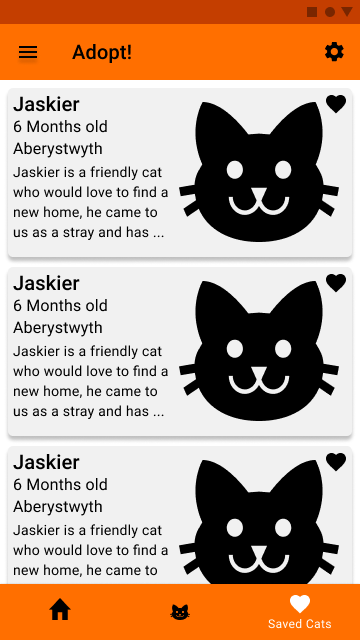
\includegraphics[height=7cm]{Images/PrototypeSavedCats.png}
    \caption{Prototype saved cats screen}
    \label{fig:prototype_saved_cats}
\end{figure}

The saved cats screen is where a user can see (once logged in) all of the cats they have favourited/saved using the heart icon found throughout the application closely associated with a cat. It displays all these cats in its \gls{Card} variation called Saved Cat Card (Section \ref{PROTOTYPESAVEDCATCARD}). Each \gls{Card} has its layer and display every single cat that has been favourited in this format even if that includes every single cat in the system.

\subsection{Saved Cat Card} \label{PROTOTYPESAVEDCATCARD}

\begin{figure} [htbp!]
    \centering
    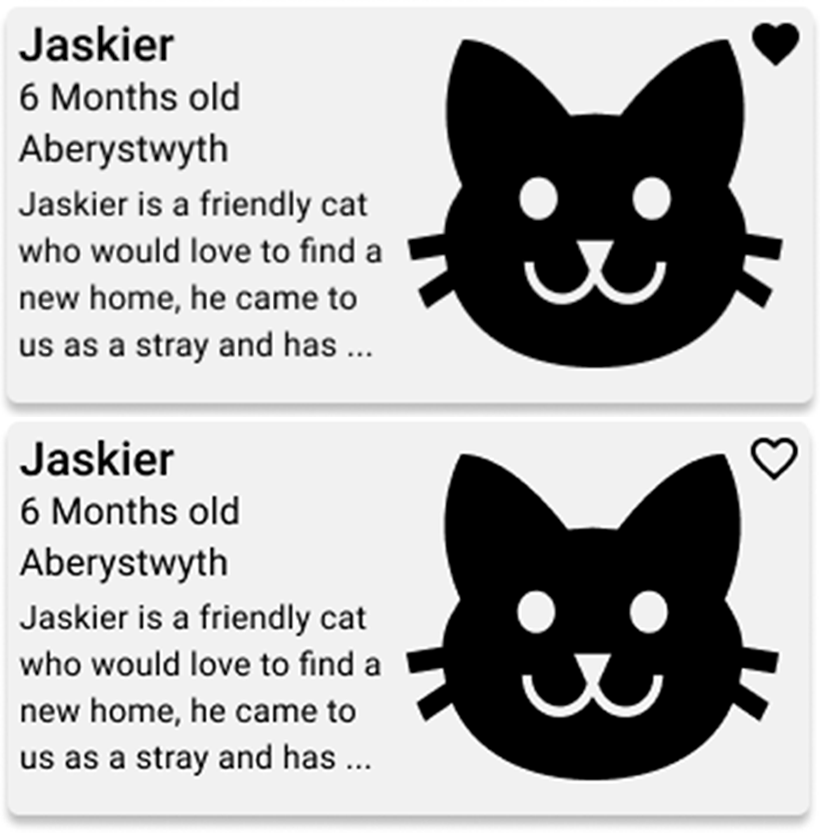
\includegraphics[height=5cm]{Images/PrototypeSavedCatCard.png}
    \caption{Prototype saved cat card}
    \label{fig:prototype_saved_cat_card}
\end{figure}

The Saved cat card is used in multiple parts of the app and is a versatile method for displaying information, it shows the start of the description for the cat, alongside its name, age, and location much like other cat cards. This \gls{Card} also shows a larger version of the cat's scaled-down image, and a favourite button represented by either an empty or full heart, depending on whether the cat has been saved or not, if saved then it is filled, if not saved then it is not filled. This \gls{Card} functions largely the same as the Cat Card (Section \ref{PROTOTYPECATCARD}).

The reason there is a more detailed card for cats of more interest is that they are of a higher interest to potential adopters than the other cats listed in the application. The other cats are not saved or featured for any specific reason, due to the volume of cats more detail can't be shown, but with these more special interest cats, they can have the attention that it requires given with this more detailed \gls{Card}.

\subsection{Adoption Status Card} \label{PROTOTYPEADOPTIONSTATUSCARD}

\begin{figure} [htbp!]
    \centering
    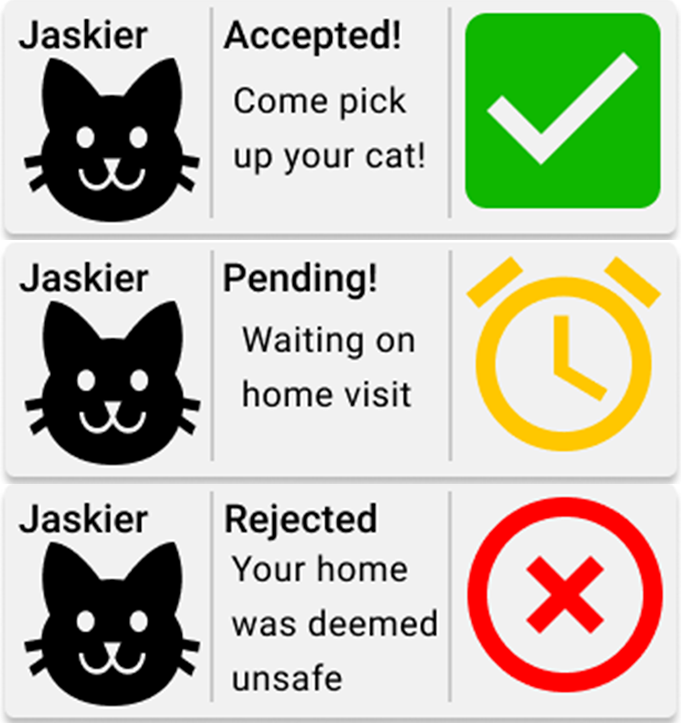
\includegraphics[height=6cm]{Images/PrototypeAdoptionCards.png}
    \caption{Prototype adoption status card}
    \label{fig:prototype_adoption_status_card}
\end{figure}

The adoption status \gls{Card} has 2 purposes, to display the current state of an adoption request, this has 3 major states, accepted, pending/being processed, and rejected. Alongside the major states, there are more nuanced details added to it, at present they are pretty basic, but if a person's application is rejected, then it says why, if a user's application is pending it says why. The \gls{Card} includes the name and picture of the cat, so a user knows which cat this adoption application is related to, as a user may have more than one adoption request, rejected or otherwise.

If you click on this \gls{Card} much like any other \gls{Card} it will expand to show more information, the information it shows is relevant to the adoption status and is discussed in section \ref{PROTOTYPEADOPTIONSTATUSINFOMATION}.

\subsection{Cat Card}\label{PROTOTYPECATCARD}

\begin{figure} [htbp!]
    \centering
    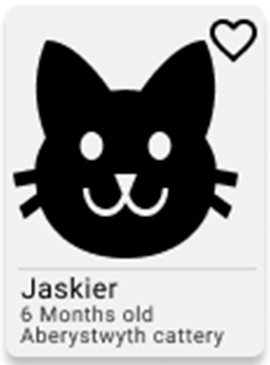
\includegraphics[height=3cm]{Images/PrototypeCatCard.png}
    \caption{Prototype cat card}
    \label{fig:prototype_cat_card}
\end{figure}

The base-level Cat \gls{Card} is the primary way a user will first see their future cats; it is the primary method from which a user is expected to interact with a cat. It's a small compact area to display essential information related to the cat. The most key information was decided to be, what the cat looked like, the name, its age, and location in that order. The order of importance for information is displayed in this Cat \gls{Card}, as top-down. The cat card does allow for quick saving/favouriting as long as a user is logged in, much like the Saved Cat \gls{Card}, by tapping the button in the top right shaped like a heart, if not filled the cat is not saved, if filled then the cat has already been saved by that user, and can be used to unsaved the cat.

If the Cat \gls{Card} is clicked/tapped then the user will be navigated to the respective cat's Cat Information screen. (Section \ref{PROTOTYPECATINFORMATIONSCREEN})
\subsection{Adoption Status Screen} \label{PROTOTYPEADOPTIONSTATUSINFOMATION}

\begin{figure} [htbp!]
    \centering
    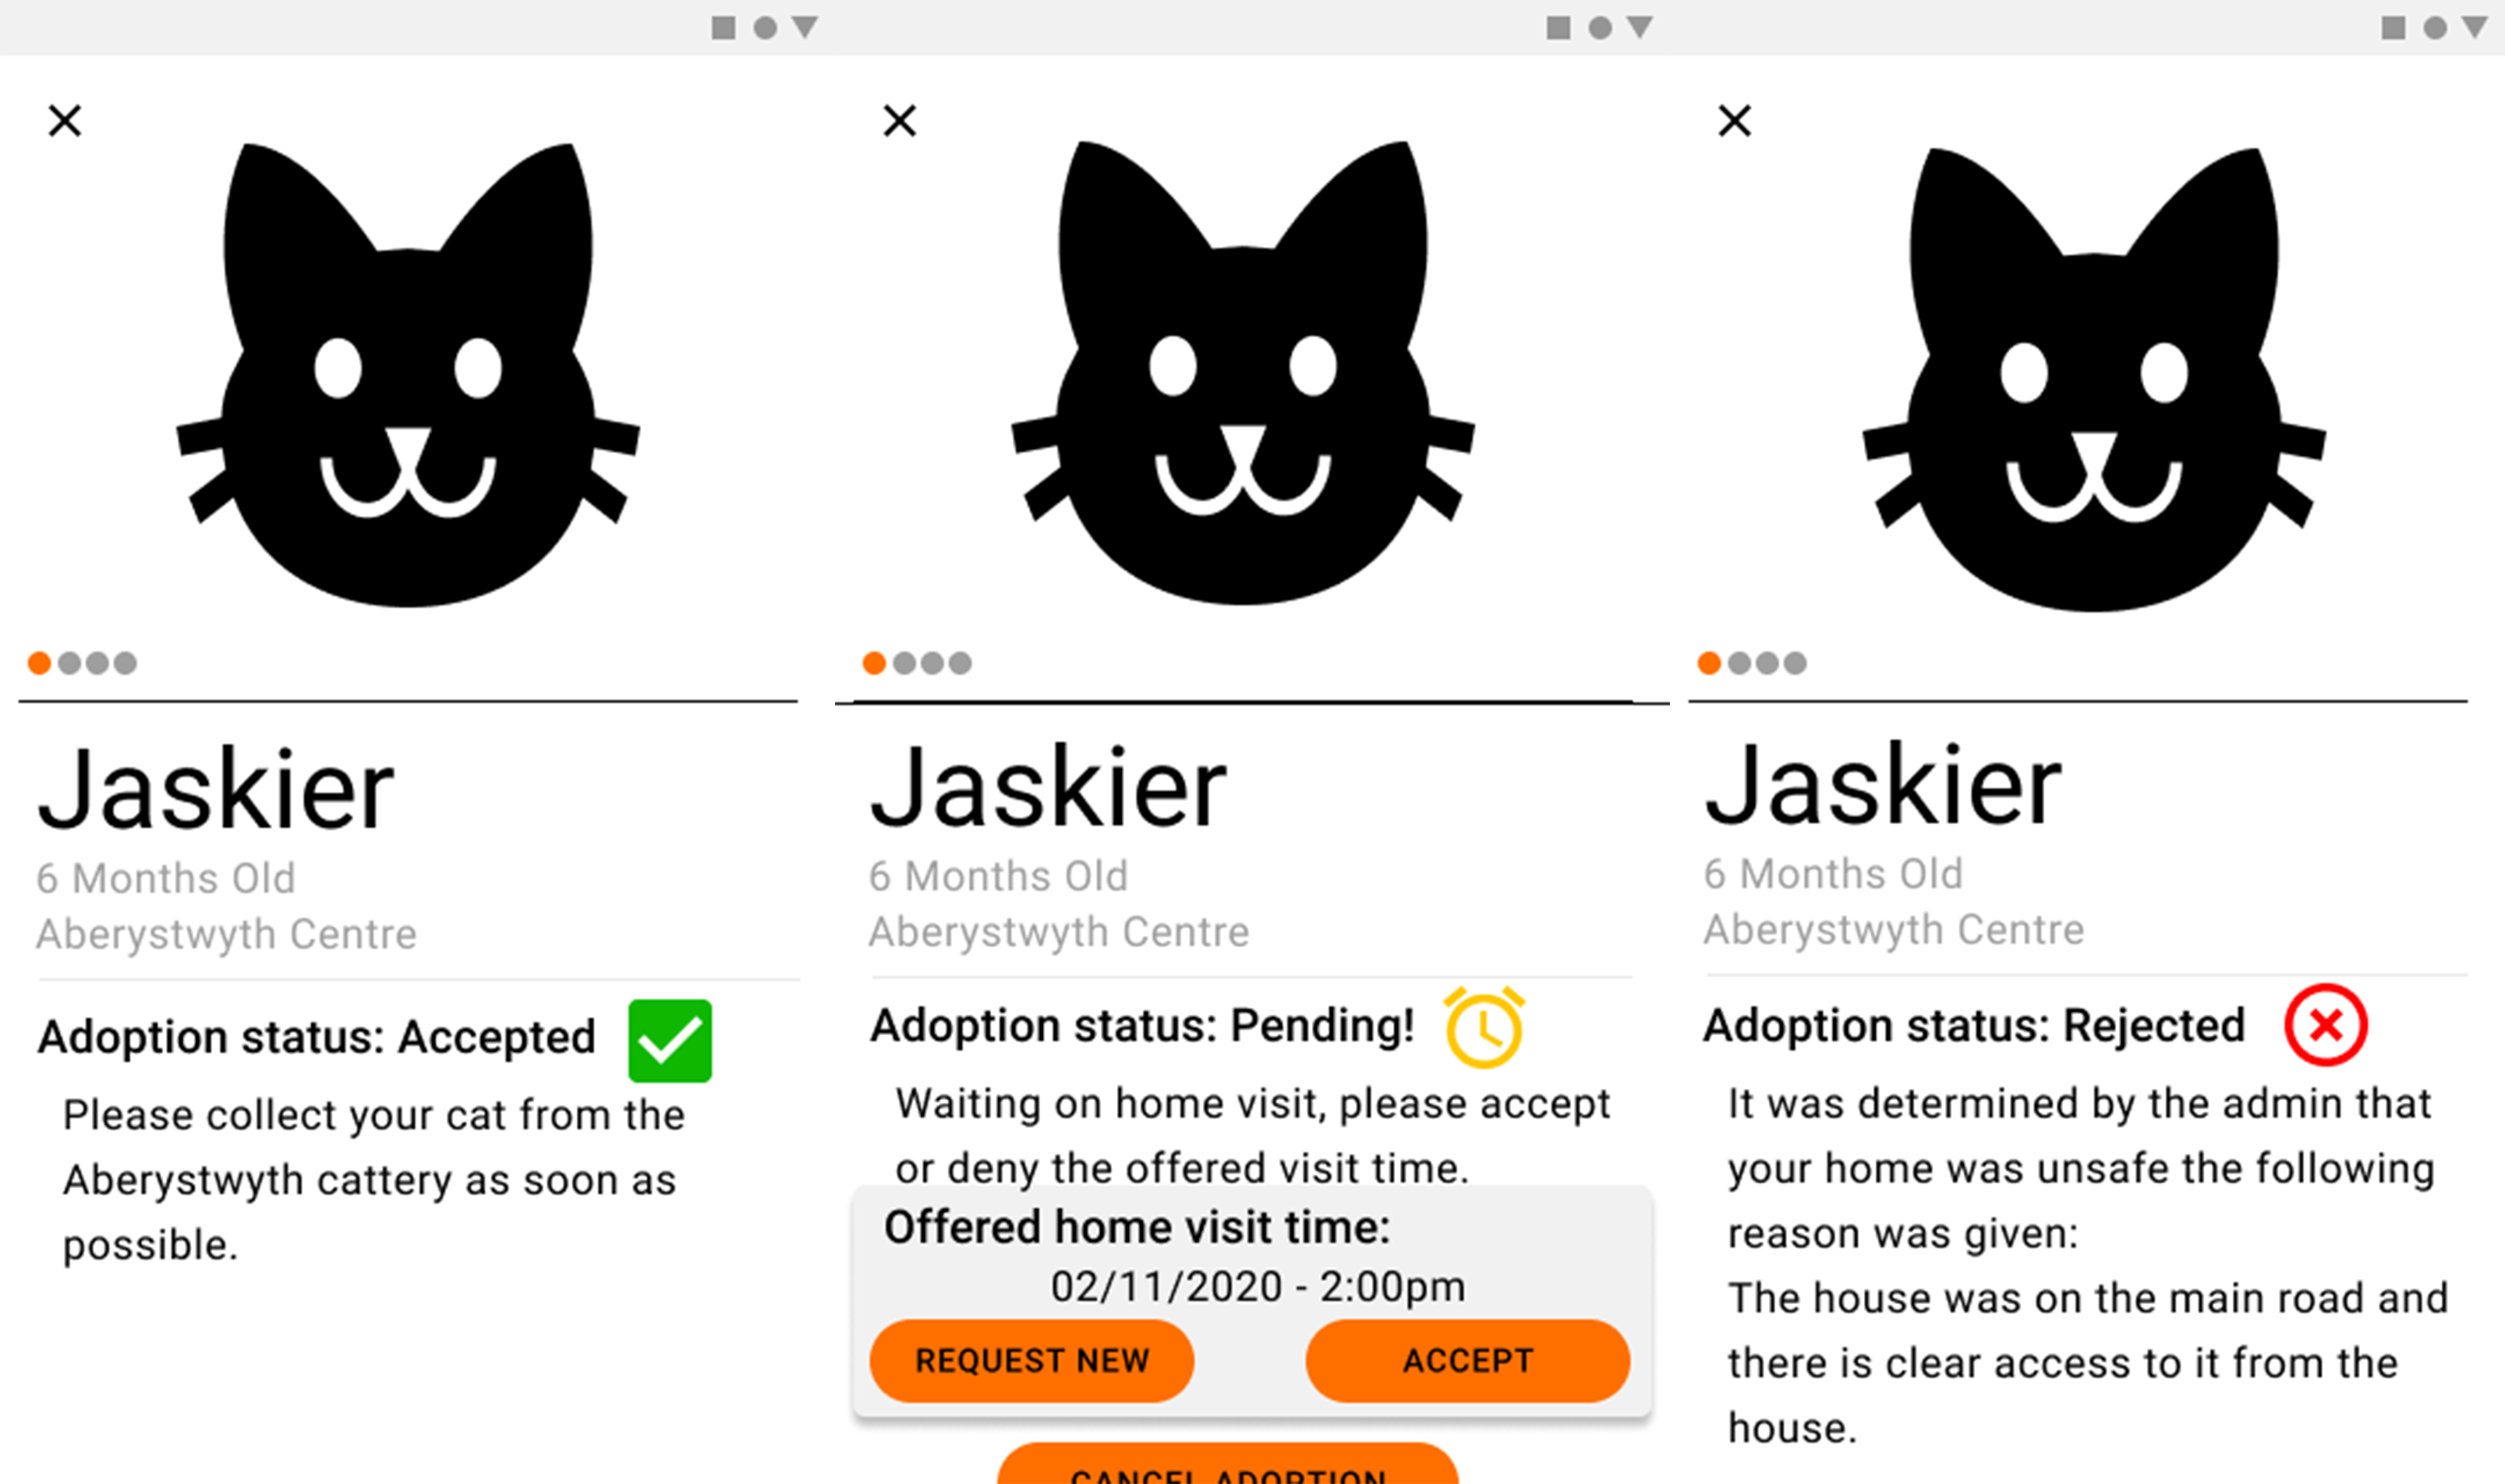
\includegraphics[height=7cm]{Images/PrototypeAdoptionStatusInfomation.png}
    \caption{Prototype more adoption information screen}
    \label{fig:prototype_adoption_status_infomation}
\end{figure}

The design for this screen is mostly the same as the prototype cat information screen (Section \ref{PROTOTYPECATINFORMATIONSCREEN}). A cross replaces the up/navigation draw button as now, and you may want to close the screen and return, it will not strictly be an up navigation as it is technically a pop-up. The cat, name, age and location are shown to reinforce to a user that they are looking at the correct cat's adoption form.

The adoption status screen portrayed in this prototype allows for the acceptance of appointments or requesting of new appointments, further details as to why your application may have been accepted, rejected, or still pending. Finally, it allows for a user to cancel their adoption request if it is still pending. Rejected ones are not removable, and neither are accepted ones, not that a user necessarily wants to do that if so it is possible outside of the application by an administrator.

\subsection{Navigation Draw} \label{PROTOTYPENAVIGATIONDRAW}

\begin{figure} [htbp!]
    \centering
    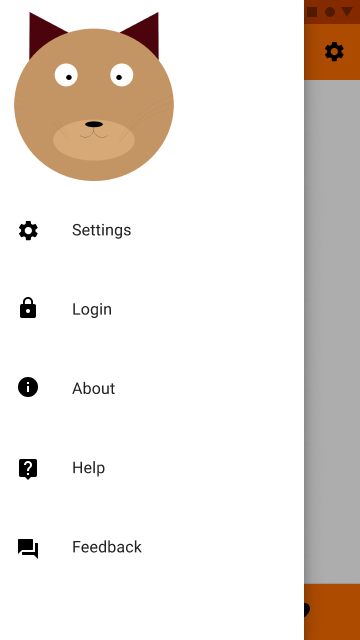
\includegraphics[height=7cm]{Images/PrototypeNavDraw.png}
    \caption{Prototype navigation draw}
    \label{fig:prototype_nav_draw}
\end{figure}

This is a prototype bare-bones navigation draw (Figure \ref{fig:prototype_nav_draw}) to allow navigation to more rarely visited parts of the app, here you can access your login/my account, about, help, and feedback screens in the application. These are not used regularly, but they do allow users access to more information from the app, the navigation draw was added in conjunction with the \gls{Bottom Navigation Bar} to allow the user to navigate to these but more hidden than the Bottom Navigation Bar.

The idea is to have the navigation draw, include a logo and below that the actual navigation locations.

\subsection{Login Screen}

\begin{figure} [htbp!]
    \centering
    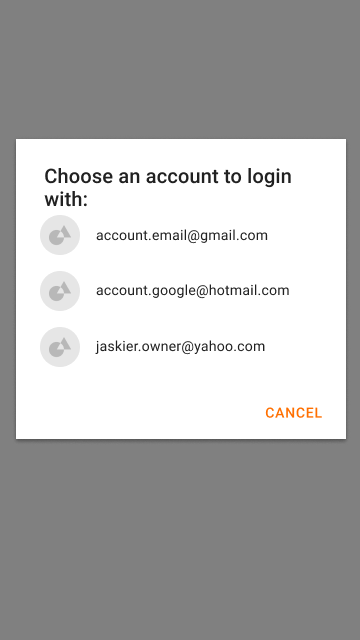
\includegraphics[height=7cm]{Images/PrototypeLoginScreen.png}
    \caption{Prototype login screen}
    \label{fig:prototype_login_screen}
\end{figure}

The screen here is a place holder (Figure \ref{fig:prototype_login_screen}). I expect this to change with the implementation of technology, at the time of designing the specific technology has not been chosen. The intention is to allow a user to login, using at least google if not different accounts.

\subsection{My Account} \label{PROTOTYPEMYACCOUNTPAGE}

\begin{figure} [htbp!]
    \centering
    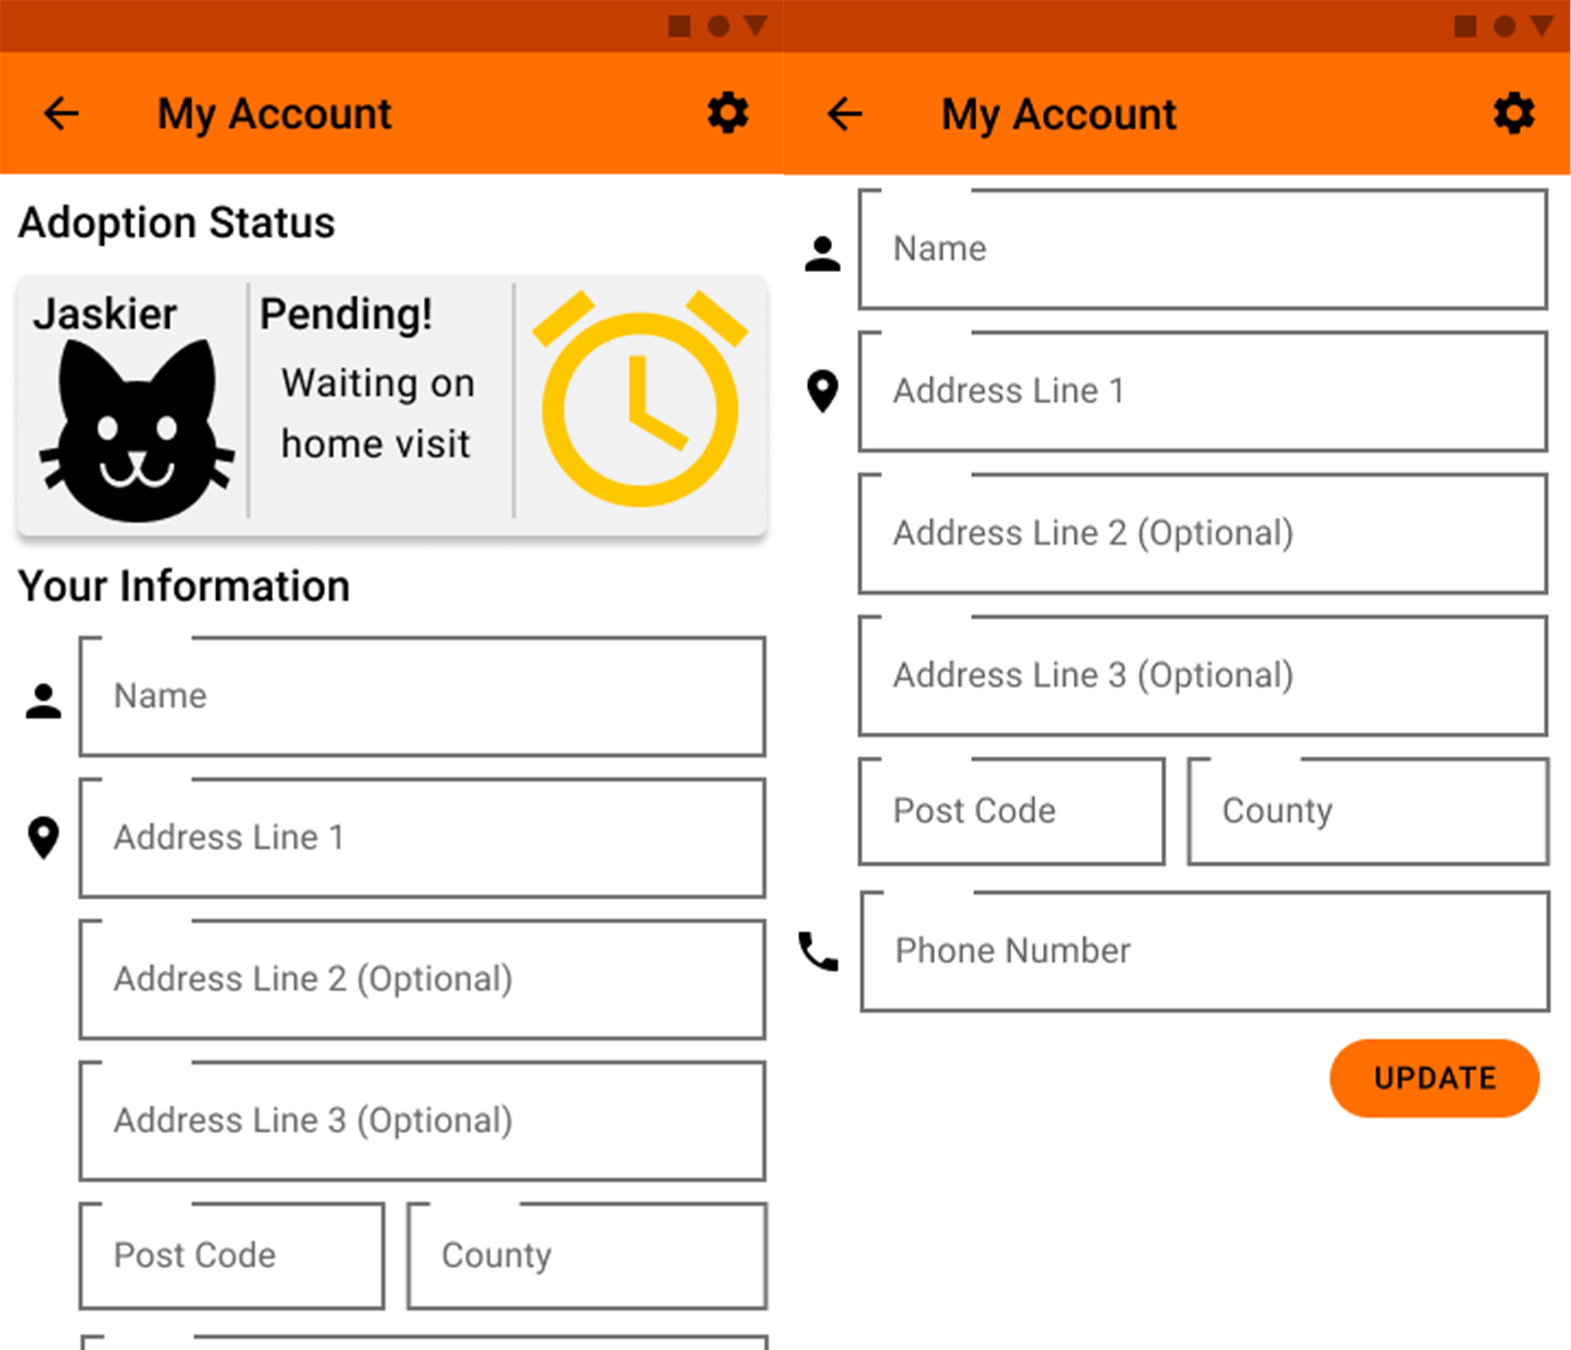
\includegraphics[height=7cm]{Images/PrototypeMyAccount.png}
    \caption{Prototype account screen}
    \label{fig:prototype_account_screen}
\end{figure}

The account screen shows current adoption statuses using the Adoption Status Cards (Section \ref{PROTOTYPEADOPTIONSTATUSCARD}), and all of them are shown in the account, even if that is not clear from the prototype. 

From this screen the users can also update their current details so an administrator can call or arrive on time to inspect the premises, these details can be updated by filling in the text fields and clicking update, it is also auto-filled by data from the database should it already be there to avoid overwriting the same data.

Ideally, there would be a place to logout here; this is done during implementation and is not shown in the prototype as it was an oversight.

\subsection{Settings}

\begin{figure} [htbp!]
    \centering
    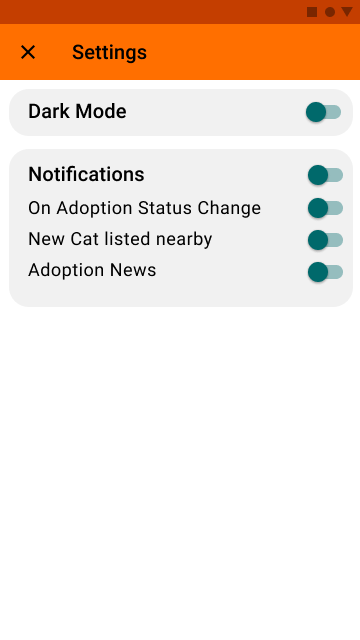
\includegraphics[height=7cm]{Images/PrototypeSettings.png}
    \caption{Prototype settings screen}
    \label{fig:prototype_settings_screen}
\end{figure}

The settings tab here is bare-bones, also it is up for debate whether or not the notifications should be in the application or not, based on the fact that Android 10 requires all of these settings to be in the system settings for this application anyway. Dark Mode is potentially system level as well but is currently only expected to work at the application level. 

Other settings can easily be added or removed based on future expansion, and this is only implemented to a basic level.

\subsection{About}

\begin{figure} [htbp!]
    \centering
    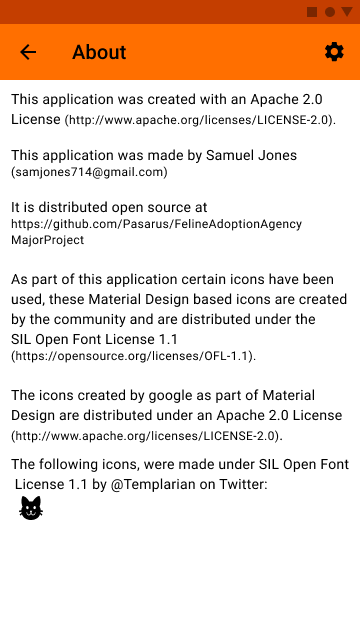
\includegraphics[height=7cm]{Images/PrototypeAbout.png}
    \caption{Prototype about screen}
    \label{fig:prototype_about_screen}
\end{figure}

The About section is a section aimed at giving the appropriate notice and thanks inside of the software for the use of software, font, and icon licenses and explicitly thanks the creators of the fonts and icons made by others in accordance with their licensing. The about page also gives the location of the distributed open-source code of the project, alongside appropriate mention of its open-source license under Apache 2.0 (\cite{APACHE2LICENSE}), this is a static page and does not change, unless via version update.

\subsection{Help}

\begin{figure} [htbp!]
    \centering
    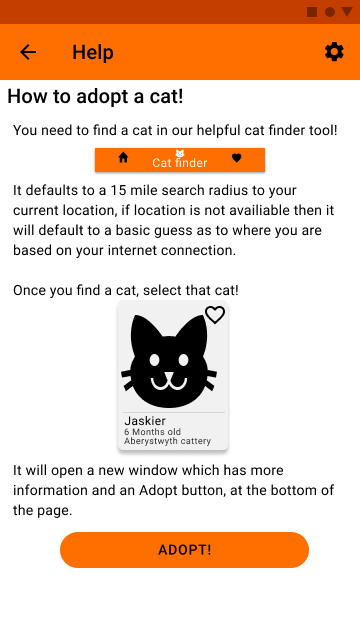
\includegraphics[height=7cm]{Images/PrototypeHelp.png}
    \caption{Prototype help screen}
    \label{fig:prototype_help_screen}
\end{figure}

The help page is another static page, and this page is intended to offer guidance to the user on how to adopt a cat and provides a basic guideline using static images and static text that should assist in the adoption of a cat.

\subsection{Feedback}

\begin{figure} [htbp!]
    \centering
    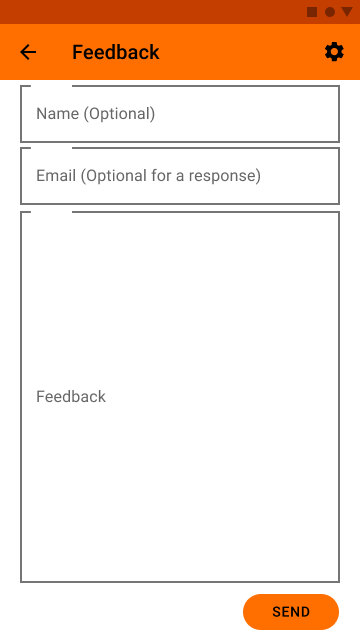
\includegraphics[height=7cm]{Images/PrototypeFeedback.png}
    \caption{Prototype feedback screen}
    \label{fig:prototype_feedback_screen}
\end{figure}

Feedback allows a logged-in user to give feedback on the application straight to the developers, and feedback can help with the applications development, a developer's awareness of bugs etc. Requiring a user to login before providing feedback is a spam avoidance mechanism, where feedback is tied to a user's identifier, meaning if they are spamming feedback from them can be easily removed and blocked from further spam.

\subsection{Cat Information Screen} \label{PROTOTYPECATINFORMATIONSCREEN}

\begin{figure} [htbp!]
    \centering
    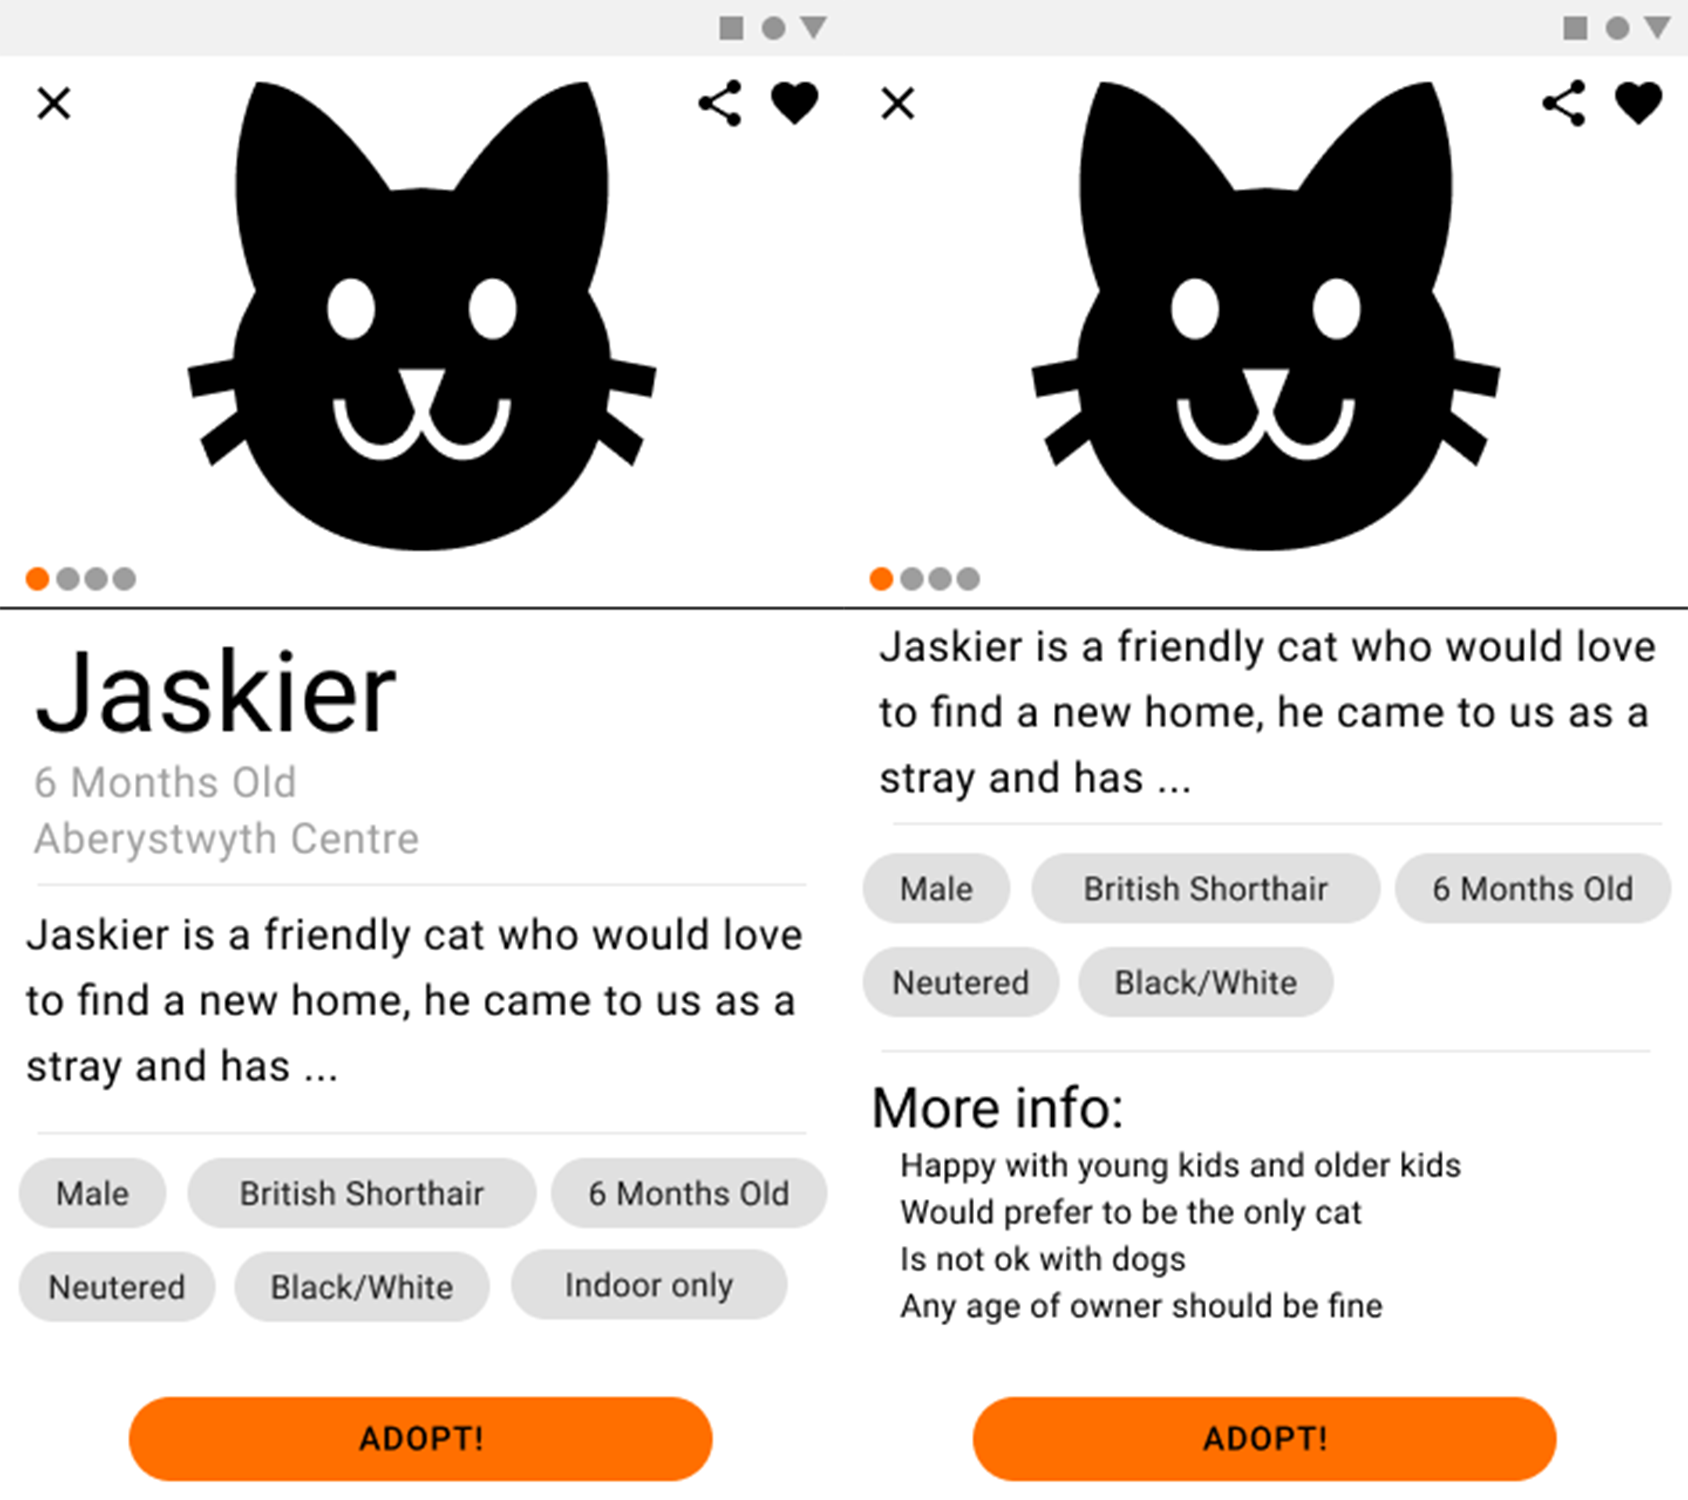
\includegraphics[height=7cm]{Images/PrototypeCatInfo.png}
    \caption{Prototype cat information screen}
    \label{fig:prototype_cat_info_screen}
\end{figure}

The cat information screen is key to showing more details to a user about a specific cat, it was inspired by Material Design Guidelines \cite{MATERIALDESIGNGUIDELINES}, for its theme and layout. It informs a user if the cat likes other cats, dogs, children of multiple different age ranges, whether it is disabled, indoors only or outside, neutered or not, breed, sex, and colour. The screen allows you to adopt the cat, as well as save or share the cat with your friends. The screen also has a description that is written by a volunteer or Foster carer that cares for the cat, and this adds some personality and more adopt-ability to the cat. 

This prototype includes multiple pictures of this one cat, and this may be infeasible later due to the fact that most freely available cat photos under creative commons or other open licenses are of individual cats and not collections of photos of one cat. The process for adding more than one cat picture should not be laborious, the limiting factor is actual images.

The screen does show the same information from the Cat \gls{Card} but it is more prominent as to follow Material Design guidelines for showing more information after interacting with a Material Design \gls{Card}.

\subsection{Adoption Form}

\begin{figure} [htbp!]
    \centering
    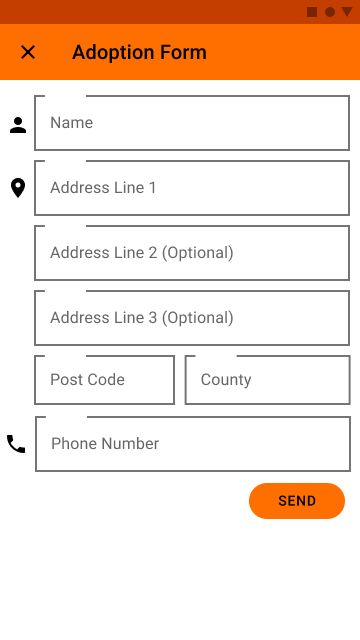
\includegraphics[height=7cm]{Images/PrototypeAdoptForm.png}
    \caption{Prototype adoption form screen}
    \label{fig:prototype_adoption_form_screen}
\end{figure}

The user must update the information in this page before adopting, before getting to this page, a user must be logged in, so the data on this page is synced with the My Account page (Section \ref{PROTOTYPEMYACCOUNTPAGE}). The reason this page must be updated is that an administrator will either ask for an appointment from the most local cattery/centre or a user should be contacted via phone, email, or mail to confirm details of the application etc. This information will be crucial to the adoption process.

\section{User interface design changes during implementation} \label{DESIGNCHANGESSECTION}
Some parts of the application have changed since the initial prototyping, and these features are detailed below in the relevant subsections. Different parts of the application prototype did not either feel right or align well with Material Design, as the project went on I reviewed and updated the designs as I implemented, reviewing the Material Design guidelines with each feature implementation \cite{MATERIALDESIGNGUIDELINES}. Some changes are not discussed here because of the nature of implementing design as an actual application and how things perform on certain devices.

\subsection{Addition of a Dark Mode Scheme}

\begin{figure} [htbp!]
    \centering
    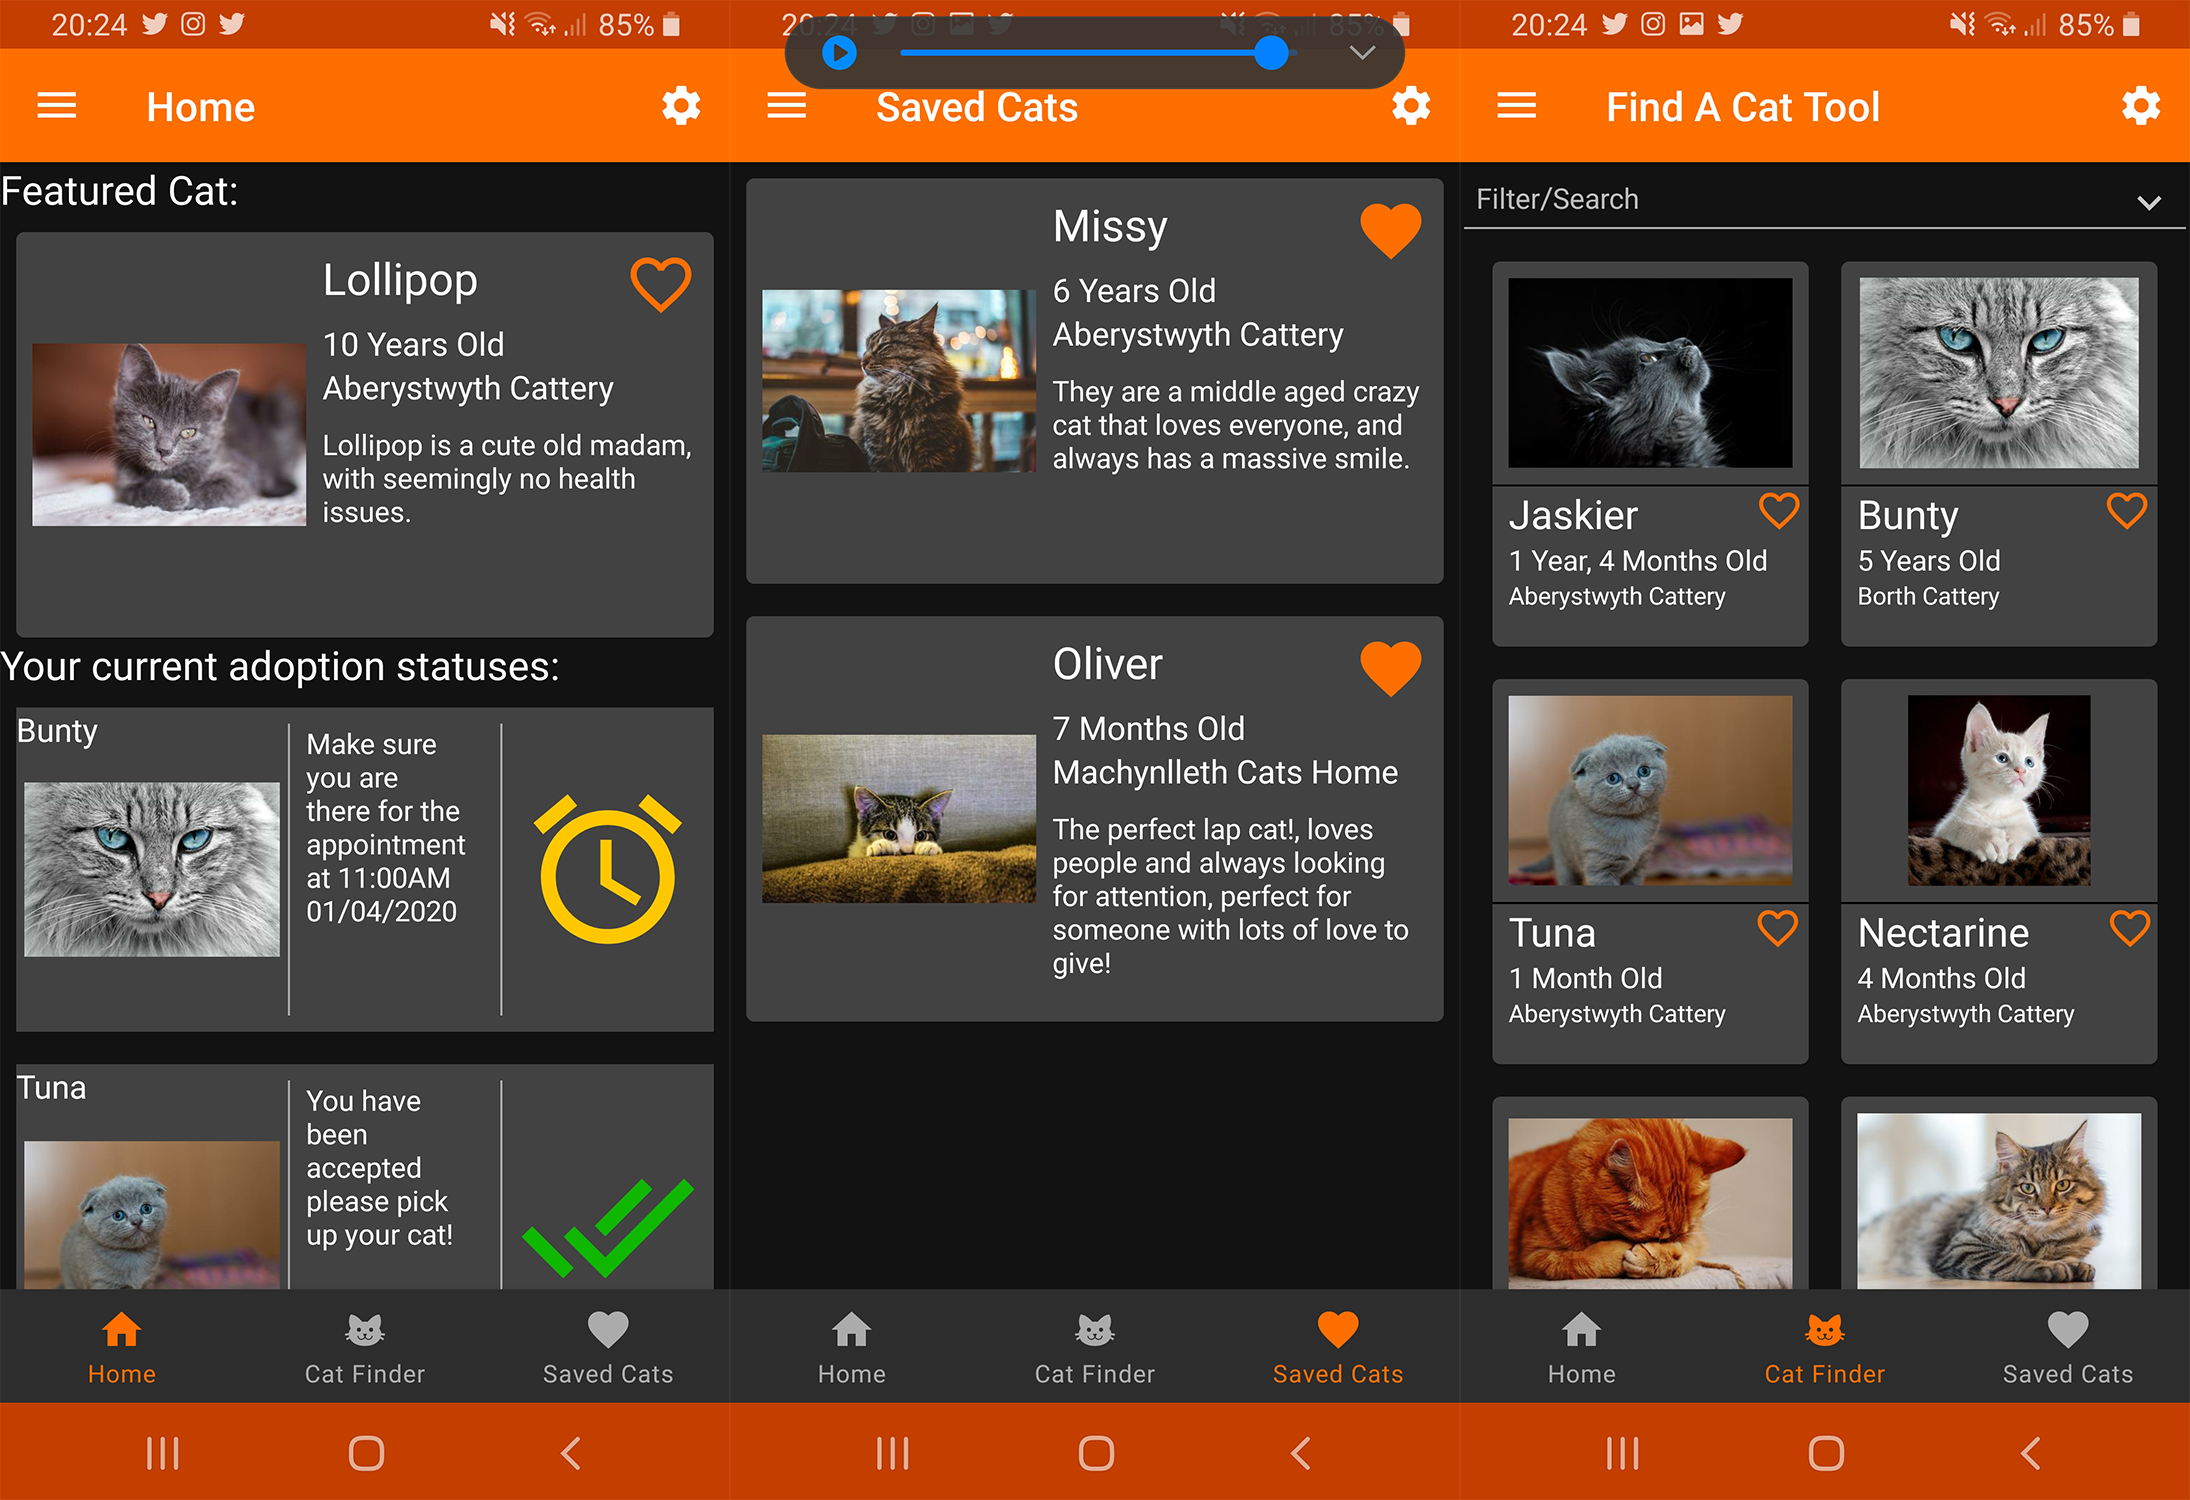
\includegraphics[height=7cm]{Images/DarkMode.png}
    \caption{Example of dark mode changes}
    \label{fig:dark_mode}
\end{figure}

During implementation it became apparent that Android developers are moving to dark mode being integrated into their application, this was addressed early in the prototype, and I believe that a darker variation of an application is often easier to use. Dark mode has been implemented using the colour scheme discussed earlier in the report in Section \ref{COLOURSCHEME}. The reason this differs from the prototype is that this was not explicitly designed in the prototype.

Dark mode is discussed in the Material Design guidelines as a feature that reduces battery drain while maintaining the same level of colour contrast. Dark themes also assist with eye strain, lowering required brightness, and allowing a user to use your application in dark areas.

\subsection{Global Navigation Structure}

\begin{figure} [htbp!]
    \centering
    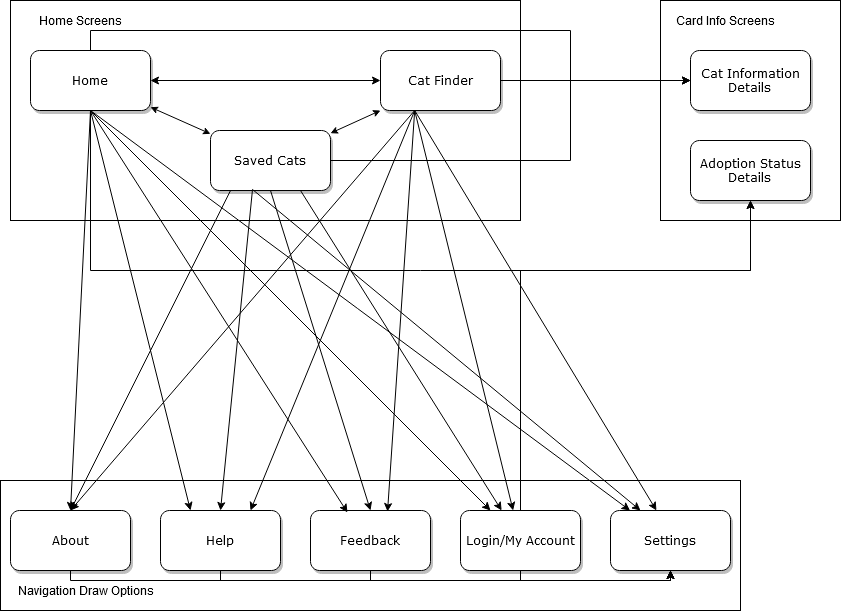
\includegraphics[width=\textwidth]{Images/Navigation Web.png}
    \caption{Theoretical navigation structure}
    \label{fig:global_structure}
\end{figure}

The global navigation structure is centred around the HomeFragment, and for usage, with the NavigationUI all screens are technically navigated to via the HomeFragment screen. However, the actual structure is designed slightly differently, for example, each \gls{Card} navigates to their respective extra information screen, not the HomeFragment, as most cards are not on the HomeFragment screen but, Cat Finder, Saved Cats, or My Account screens. You can see the theoretical navigation web at figure \ref{fig:global_structure}.

\subsection{Bottom Navigation Bar Colour Change}

\begin{figure} [htbp!]
    \centering
    
\includegraphics[height=2cm]{Images/BottomNavigationBar.png}
    \caption{Implementation of Bottom Navigation Bar}
    \label{fig:bottom_navigation_bar}
\end{figure}

In an attempt to stick strictly to Material Design guidelines with colour, the original \gls{Bottom Navigation Bar} from the earlier prototype versions that can be seen in multiple figures throughout this chapter, we have to change the design in order to portray a light and dark theme accurately. The bottom navigation bar was changed to a white background, with the primary colour as the way of determining which navigation location has been selected. All other icons from the one that is selected are greyed out. This is visible in Figure \ref{fig:bottom_navigation_bar}.

\subsection{Cat Finder Layout and Cat Card}

\begin{figure} [htbp!]
    \centering
    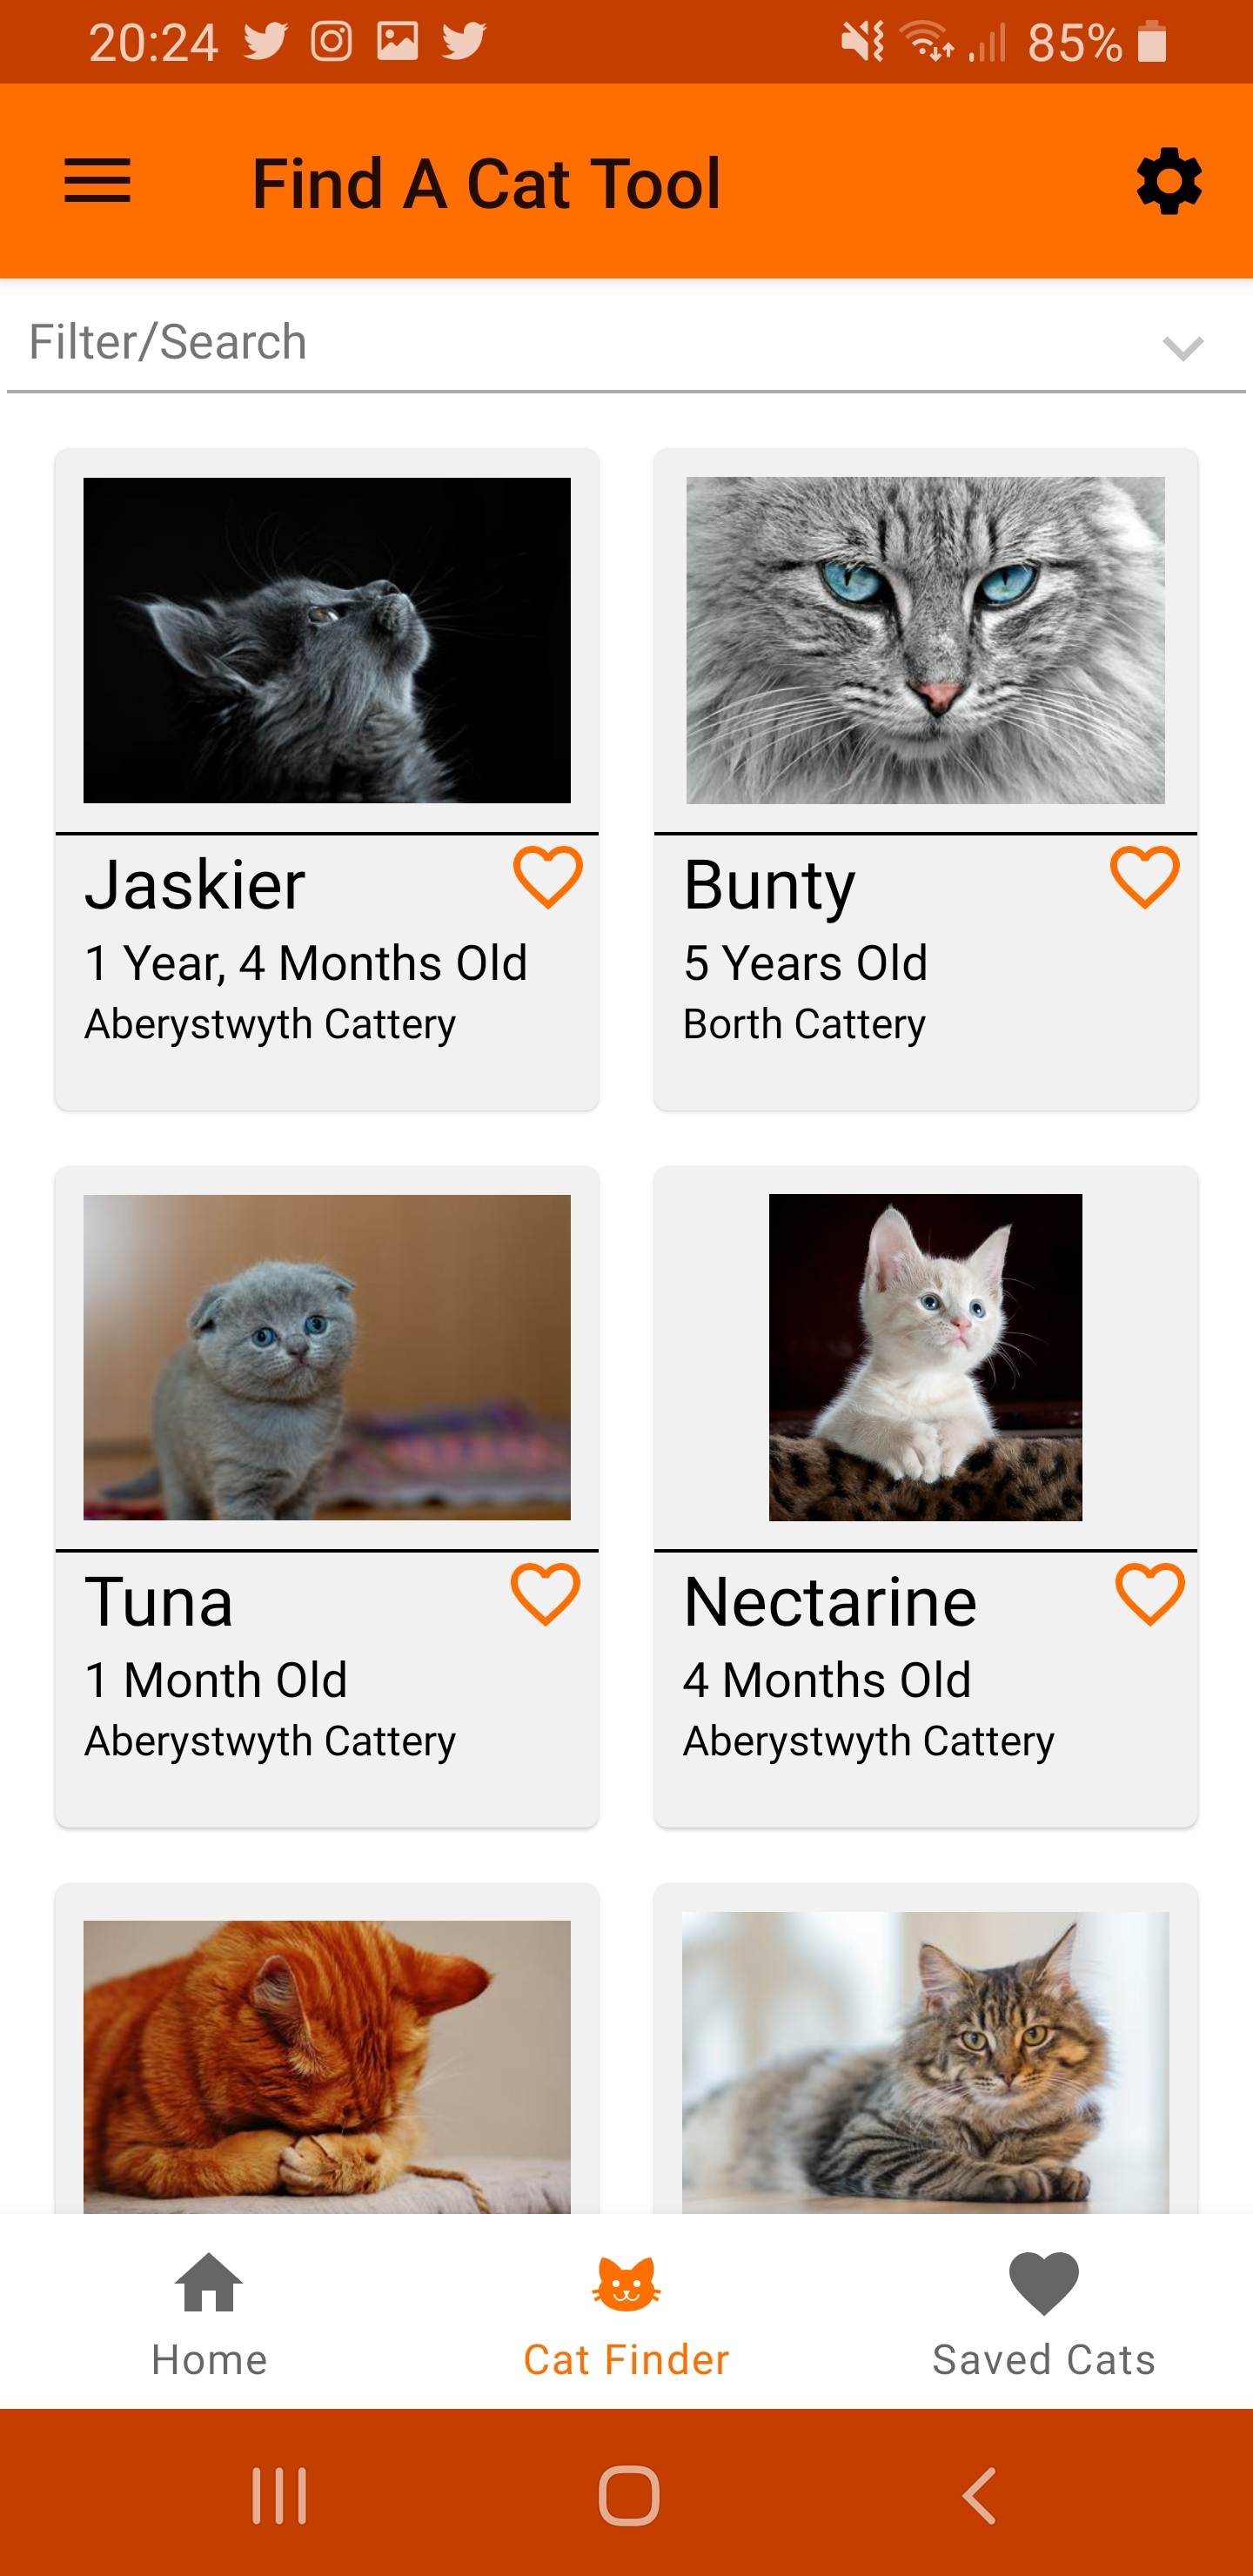
\includegraphics[height=7cm]{Images/CatFinderScreen.jpg}
    \caption{Implementation of Cat Finder}
    \label{fig:cat_finder}
\end{figure}

\begin{figure} [htbp!]
    \centering
    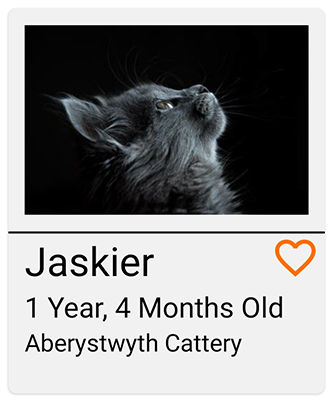
\includegraphics[height=3cm]{Images/CatCard.png}
    \caption{Cat card}
    \label{fig:cat_card}
\end{figure}

When implemented onto an actual phone the original prototype design didn't work, the text on the Cat \gls{Card} was too small, which made the layout unusable. To fix this, the Cat Card was enlarged, and it's content with it. The number of cat cards shown in a row was reduced to 2 to allow for the larger \gls{Card}s.

The Cat \gls{Card} layout also did not work very well in practice, in the prototype the favourite button was in the top right of the card over the image, this works if all images are white or transparent. Without a white or transparent background the icon could become invisible or hard to see, this lead to the slight redesign where it is on parallel with the name of the cat, it works the same as it did in the prototype.

\subsection{Saved Cats Card}

\begin{figure} [htbp!]
    \centering
    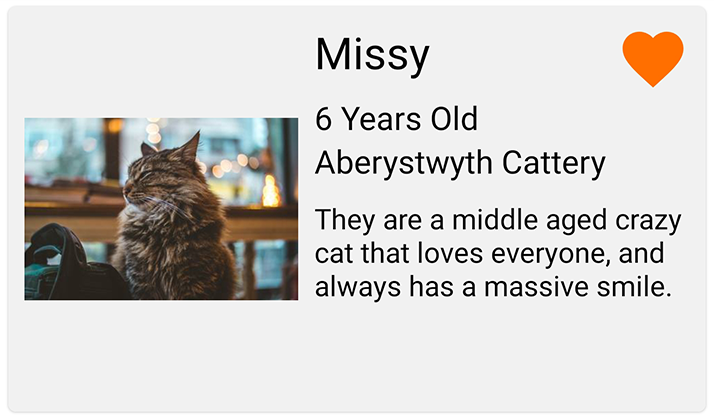
\includegraphics[height=3cm]{Images/SavedCatCard.png}
    \caption{Saved cat card}
    \label{fig:saved_cat_card}
\end{figure}

During implementation, it became apparent that the card was not designed to Material Design guidelines \cite{MATERIALDESIGNGUIDELINES}, the typical \gls{Card} in the guidelines has the image on the left, with the primary information and maybe a bit extra smaller near the bottom on the right side. To keep to this general guideline, I redesigned the Saved Cat \gls{Card}. This new layout should be quicker to glance at due to only needing the image to recognise which cat is which. This design flips if the user is using a right to left layout on Android.

\subsection{Adoption Confirmation Screen}

\begin{figure} [htbp!]
    \centering
    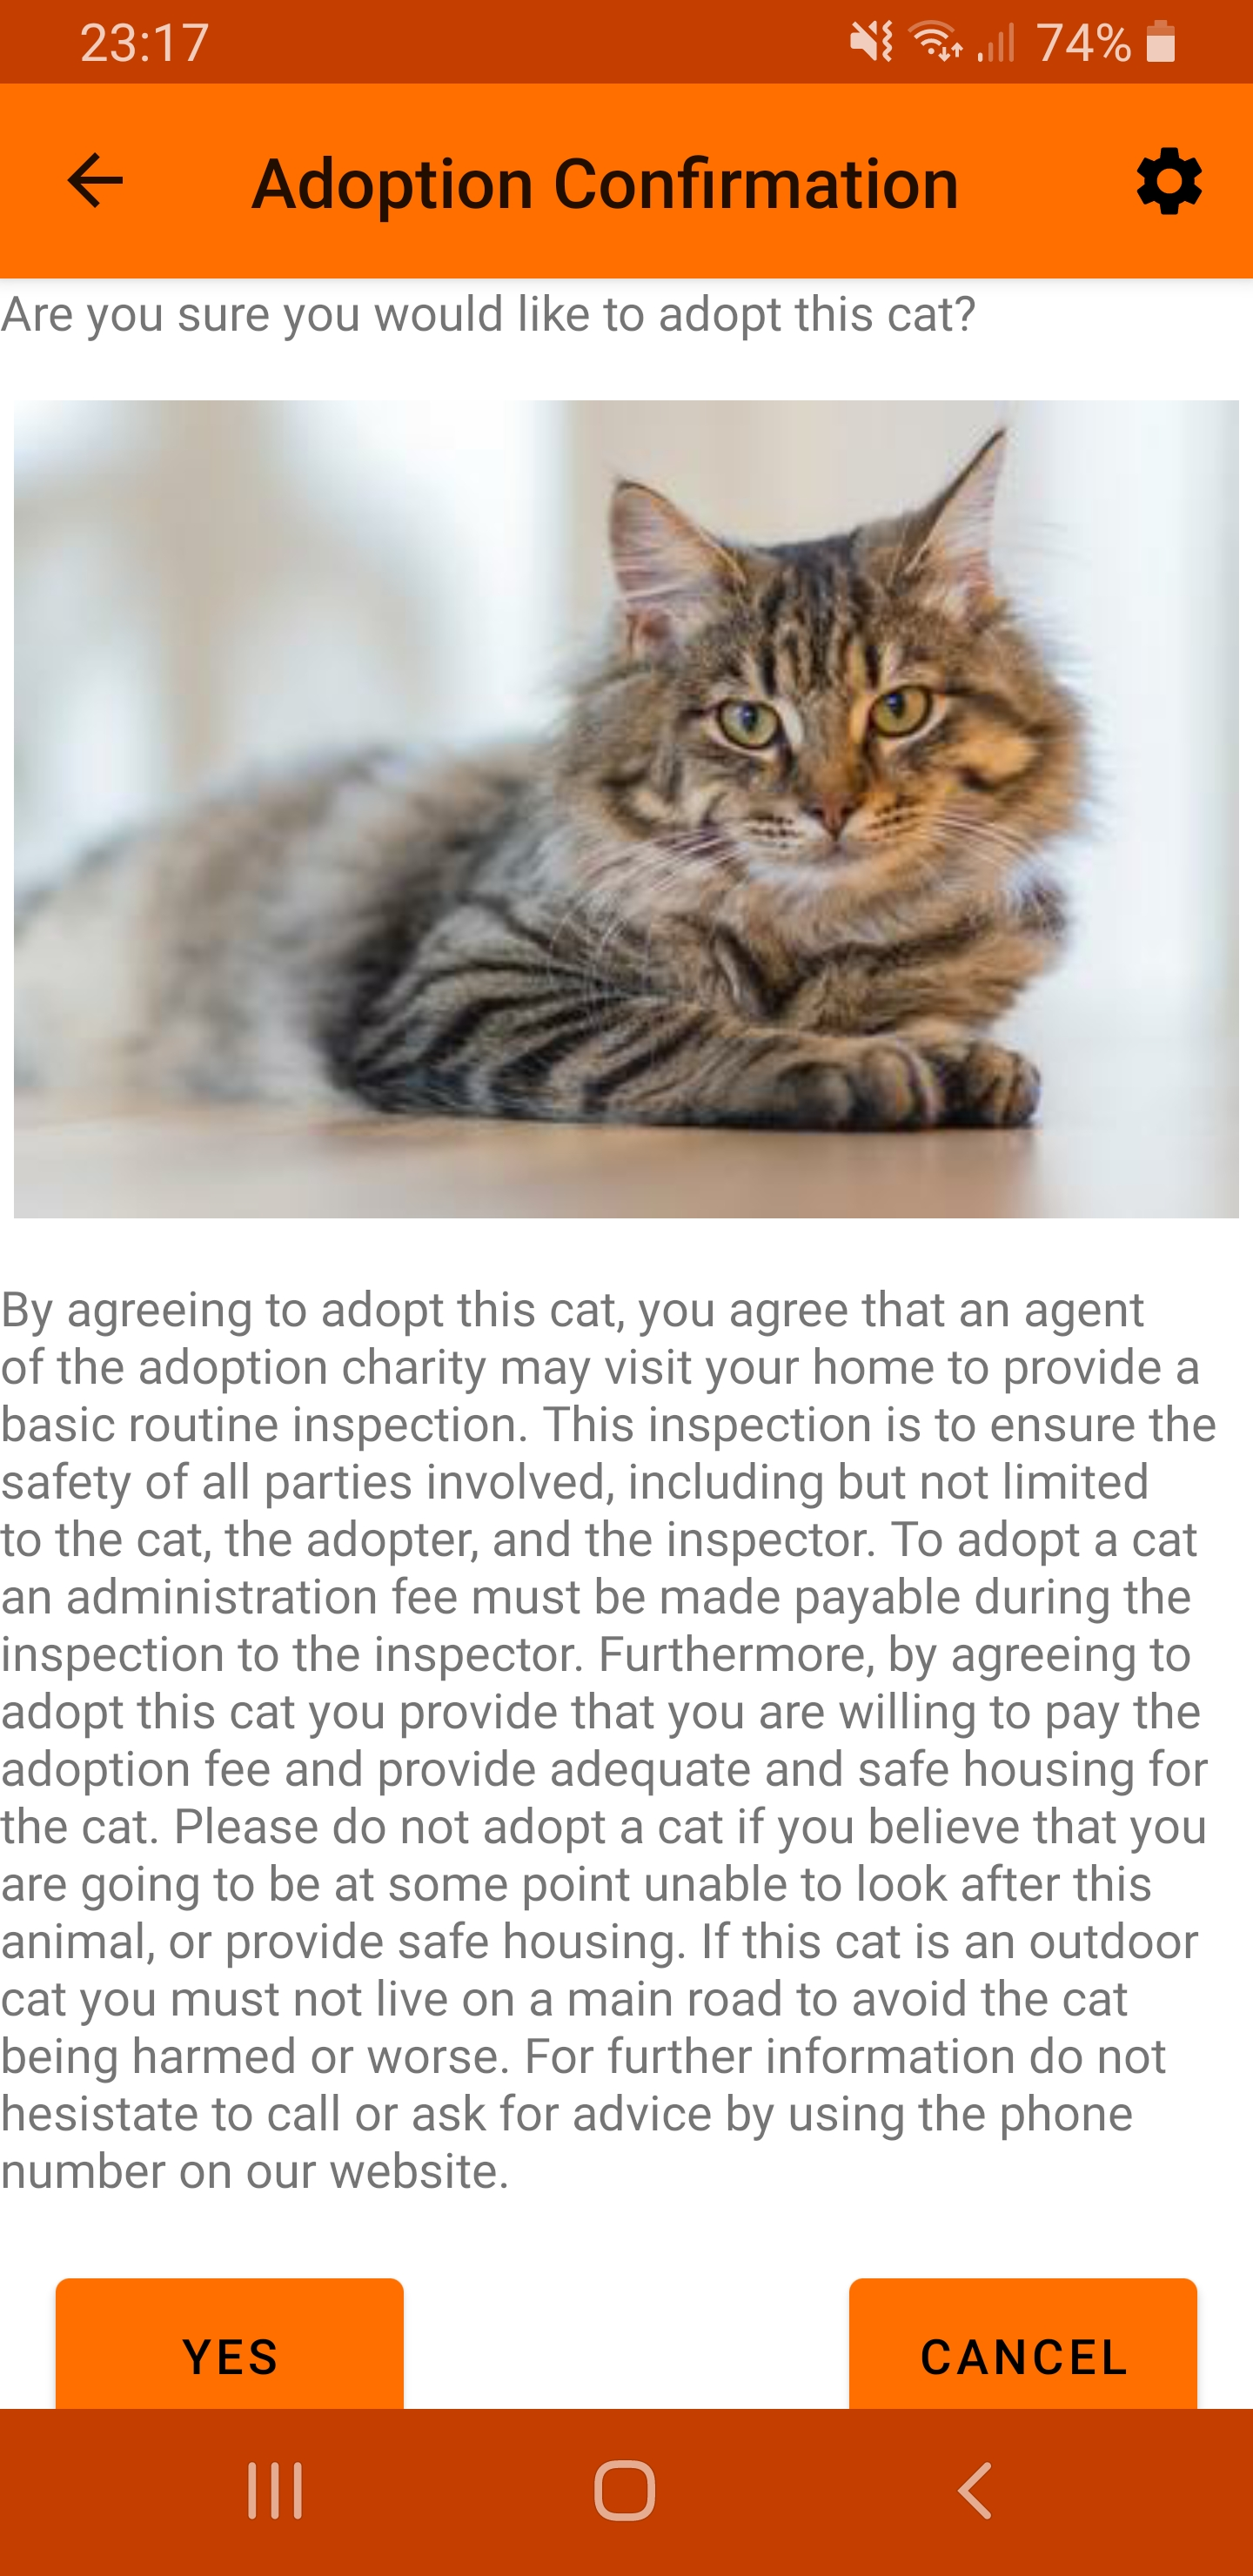
\includegraphics[height=7cm]{Images/AdoptionConfirmationScreen.jpg}
    \caption{Adoption confirmation screen}
    \label{fig:adoption_confirmation_screen}
\end{figure}

The adoption confirmation screen was added as a necessity to make sure a user is sure they want to start the adoption process. It was added later in the development process because of when clicking update on the information form that appears after being logged in and clicking adopt, it isn't apparent to a user that they have started the process necessarily. This screen adds some much-needed clarity, as once you click that yes button, you start the process, or by clicking the cancel button effectively cancelling the process.

\subsection{Settings}

\begin{figure} [htbp!]
    \centering
    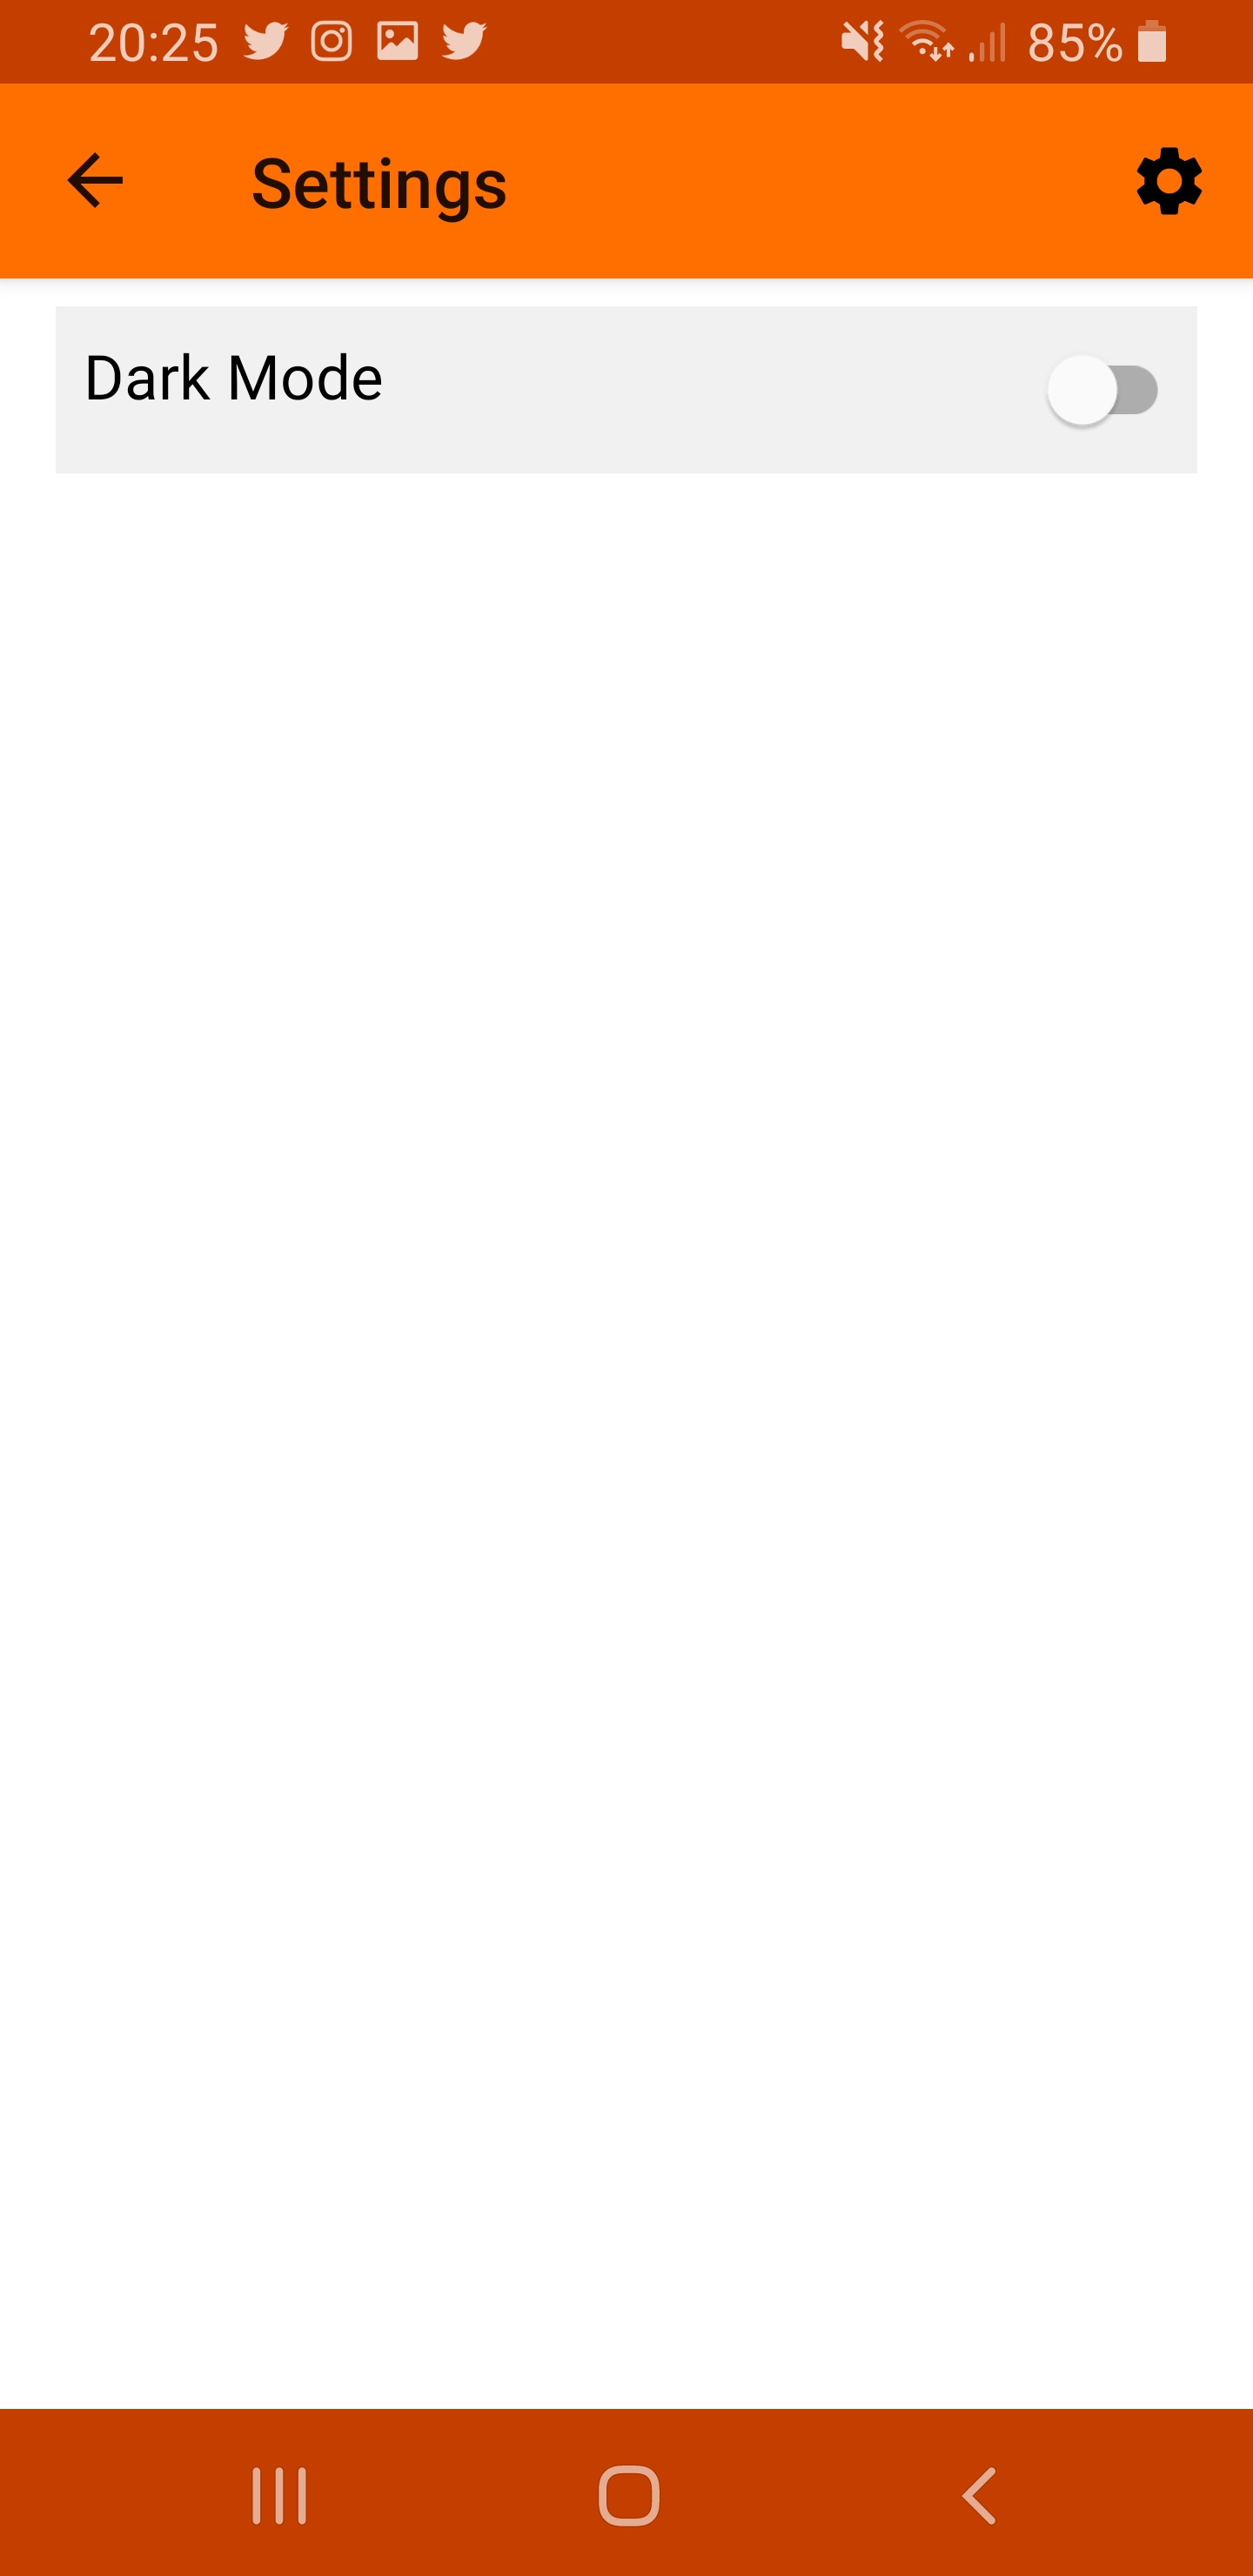
\includegraphics[height=7cm]{Images/SettingsScreen.jpg}
    \caption{Settings screen}
    \label{fig:settings_screen}
\end{figure}

The prototype settings menu contained a section for notifications, the final settings do not for two reasons, due to time constraints the notifications while present is not changeable from inside of the settings screen of the application. The second reason is, in more recent versions of Android it is possible to change these exact settings in the App info, it is also possible in all versions of Android to reject notifications from an application. 

While the prototype had green buttons, this did not follow the Material Design guidelines and was an oversight, so they were replaced to follow the guidelines with the correct colouring to represent the different states of the switches. The original prototype also had a cross instead of the up button on the upper left corner of the app while in the settings, this was switched to an up button in line with the Material Design guidelines for navigation.

\subsection{Navigation Draw}

\begin{figure} [htbp!]
    \centering
    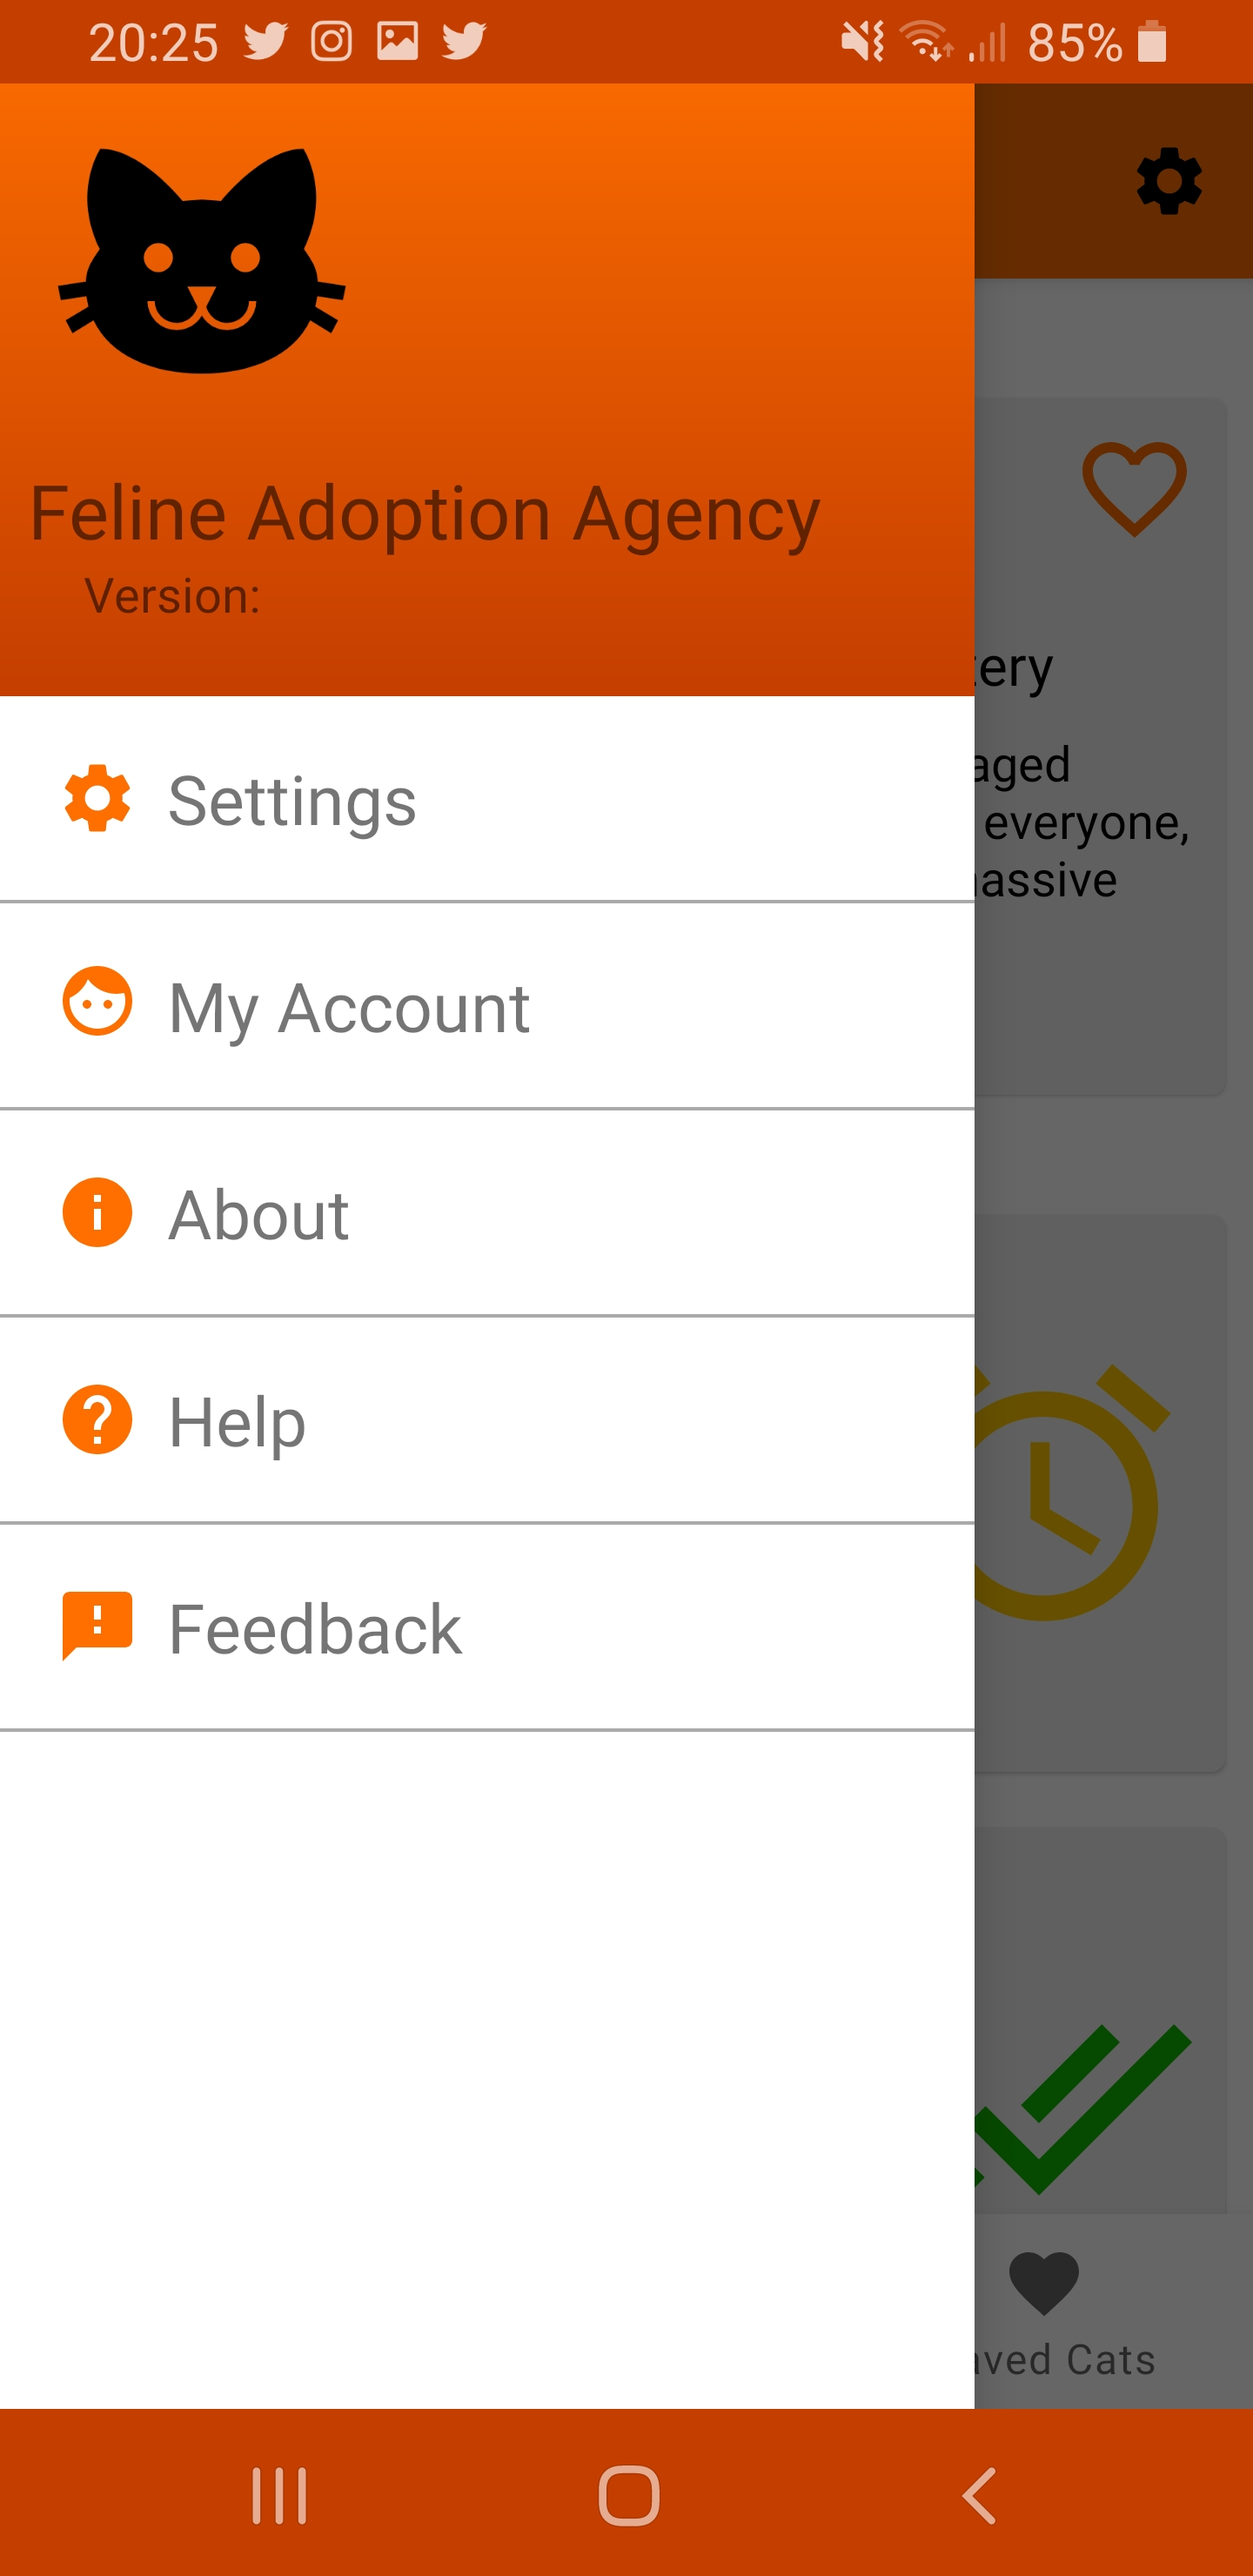
\includegraphics[height=7cm]{Images/NavigationScreen.jpg}
    \caption{Navigation draw}
    \label{fig:navigation_draw}
\end{figure}

The prototype navigation draw (Section \ref{PROTOTYPENAVIGATIONDRAW}) was never intended to be a final product or close to the final product. The final navigation draw (Figure \ref{fig:navigation_draw}) is a far superior design for multiple reasons, including the fact it makes more use of the primary colour scheme, it is interactive based on the state of the application (Login being replaced with My Account and a picture provided by the account logged in with), and it has a nicer header than just the logo that is shown in the prototype.

\subsection{Notifications}

\begin{figure} [htbp!]
    \centering
    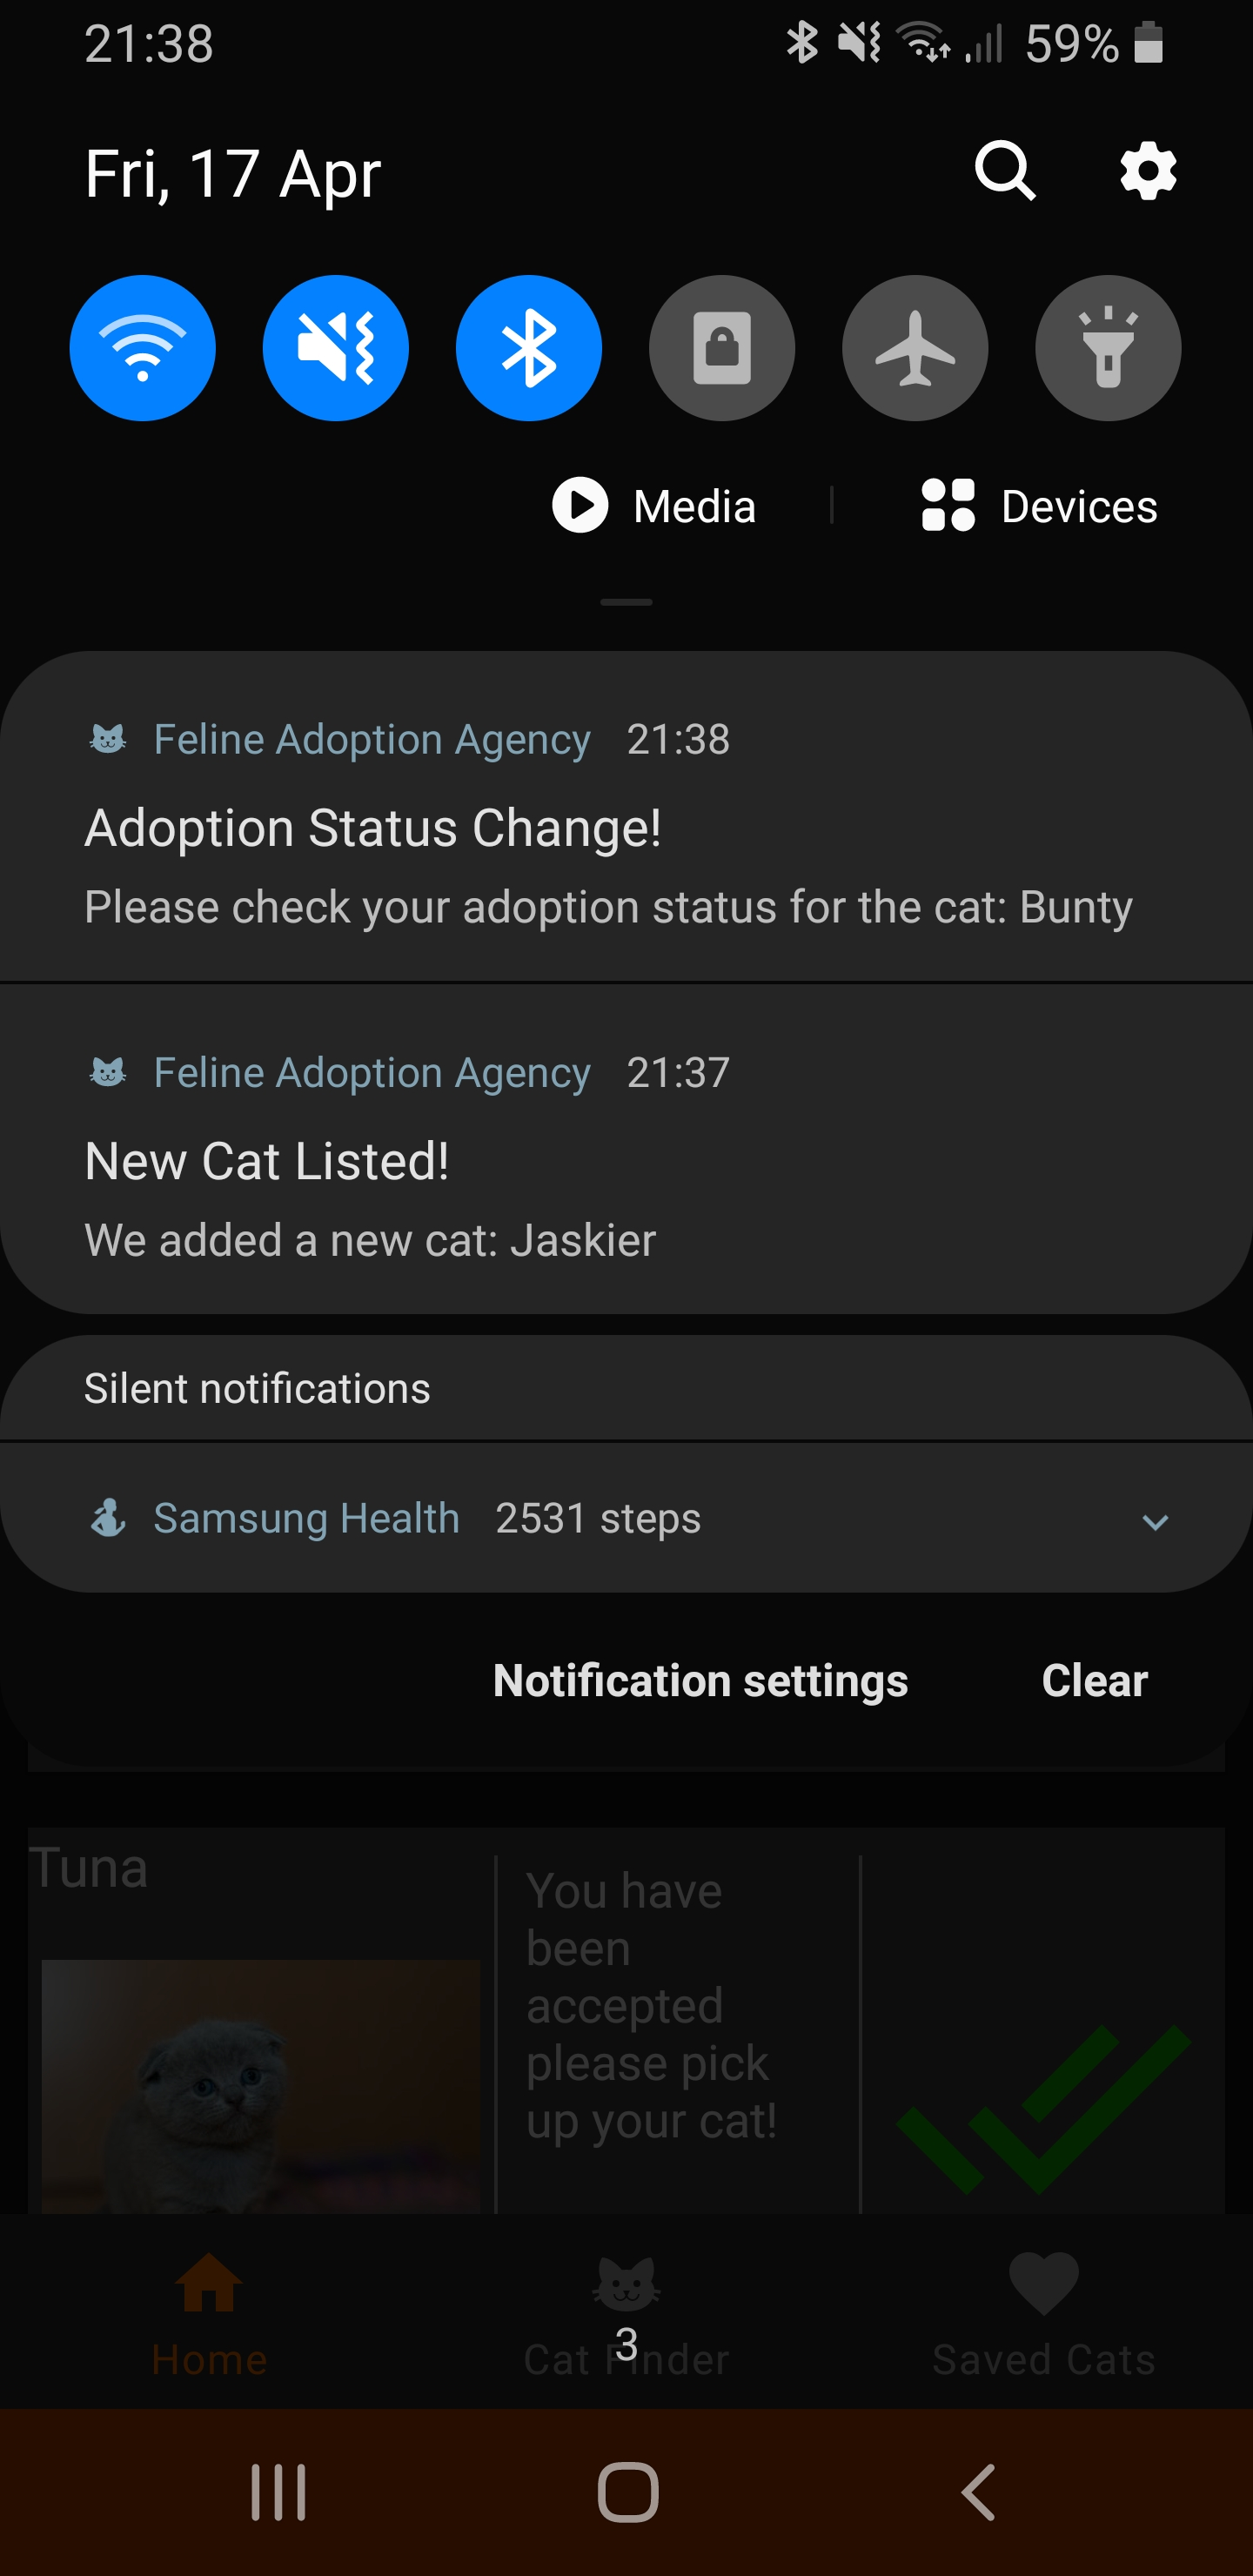
\includegraphics[height=7cm]{Images/Notifications.jpg}
    \caption{Notifications from the Feline Adoption Agency}
    \label{fig:notifications}
\end{figure}
The prototype never discussed how notifications would appear on a user's phone, and the basic Android notification pops up with a small image and with text,
 that is the exact implementation design that was completed, as shown in Figure \ref{fig:notifications}. Notifications pop up when a user's adoption status changes, a new cat is added, and some news from the agency is announced.

\section{Architecture} \label{CODESTRUCTUREDESIGN}

This section is an attempt at explaining to the reader how the UI Design and the code inside of the application fit together. Furthermore, this chapter goes into detail about how different components of the application fit together and what components there are.

\subsection{Overall Architecture}

The overall architecture of the application revolves around the theory of one activity, many fragments, this is the preferred method of application implementation \cite{SINGLEACTIVITYAPP}. The main application relies on Android Jetpack NavigationUI \cite{NAVIGATIONUI}, to navigate between fragments in the application. It is possible to pass a Java Parcelable object between fragments for data transfer, during navigation.

    \begin{figure} [htbp!]
        \centering
        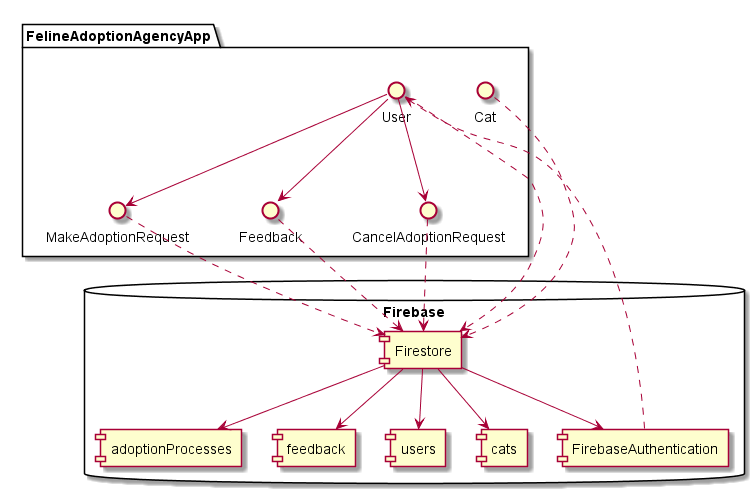
\includegraphics[width=\textwidth]{Images/ComponentDiagram.png}
        \caption{UML Component Diagram}
        \label{fig:component_diagram}
    \end{figure}
    
So far, we have not thought about how data gets to and from the application. For this, I intended to use Google's Firebase Firestore for databases using a NoSQL structure with JSON files, Firebase Authentication for authenticating a user's identity and storing of user account identifiers, and Firebase File-storage for storing pictures of cats at a URL location so the application over the internet can load them. Figure \ref{fig:component_diagram} displays the rough interactions between the app and the Firebase, inside it has the Firestore, which is the database, and the authentication of users.

    %Sequence Diagram should be added
    \begin{landscape}
        \begin{figure} [htbp!]
            \centering
            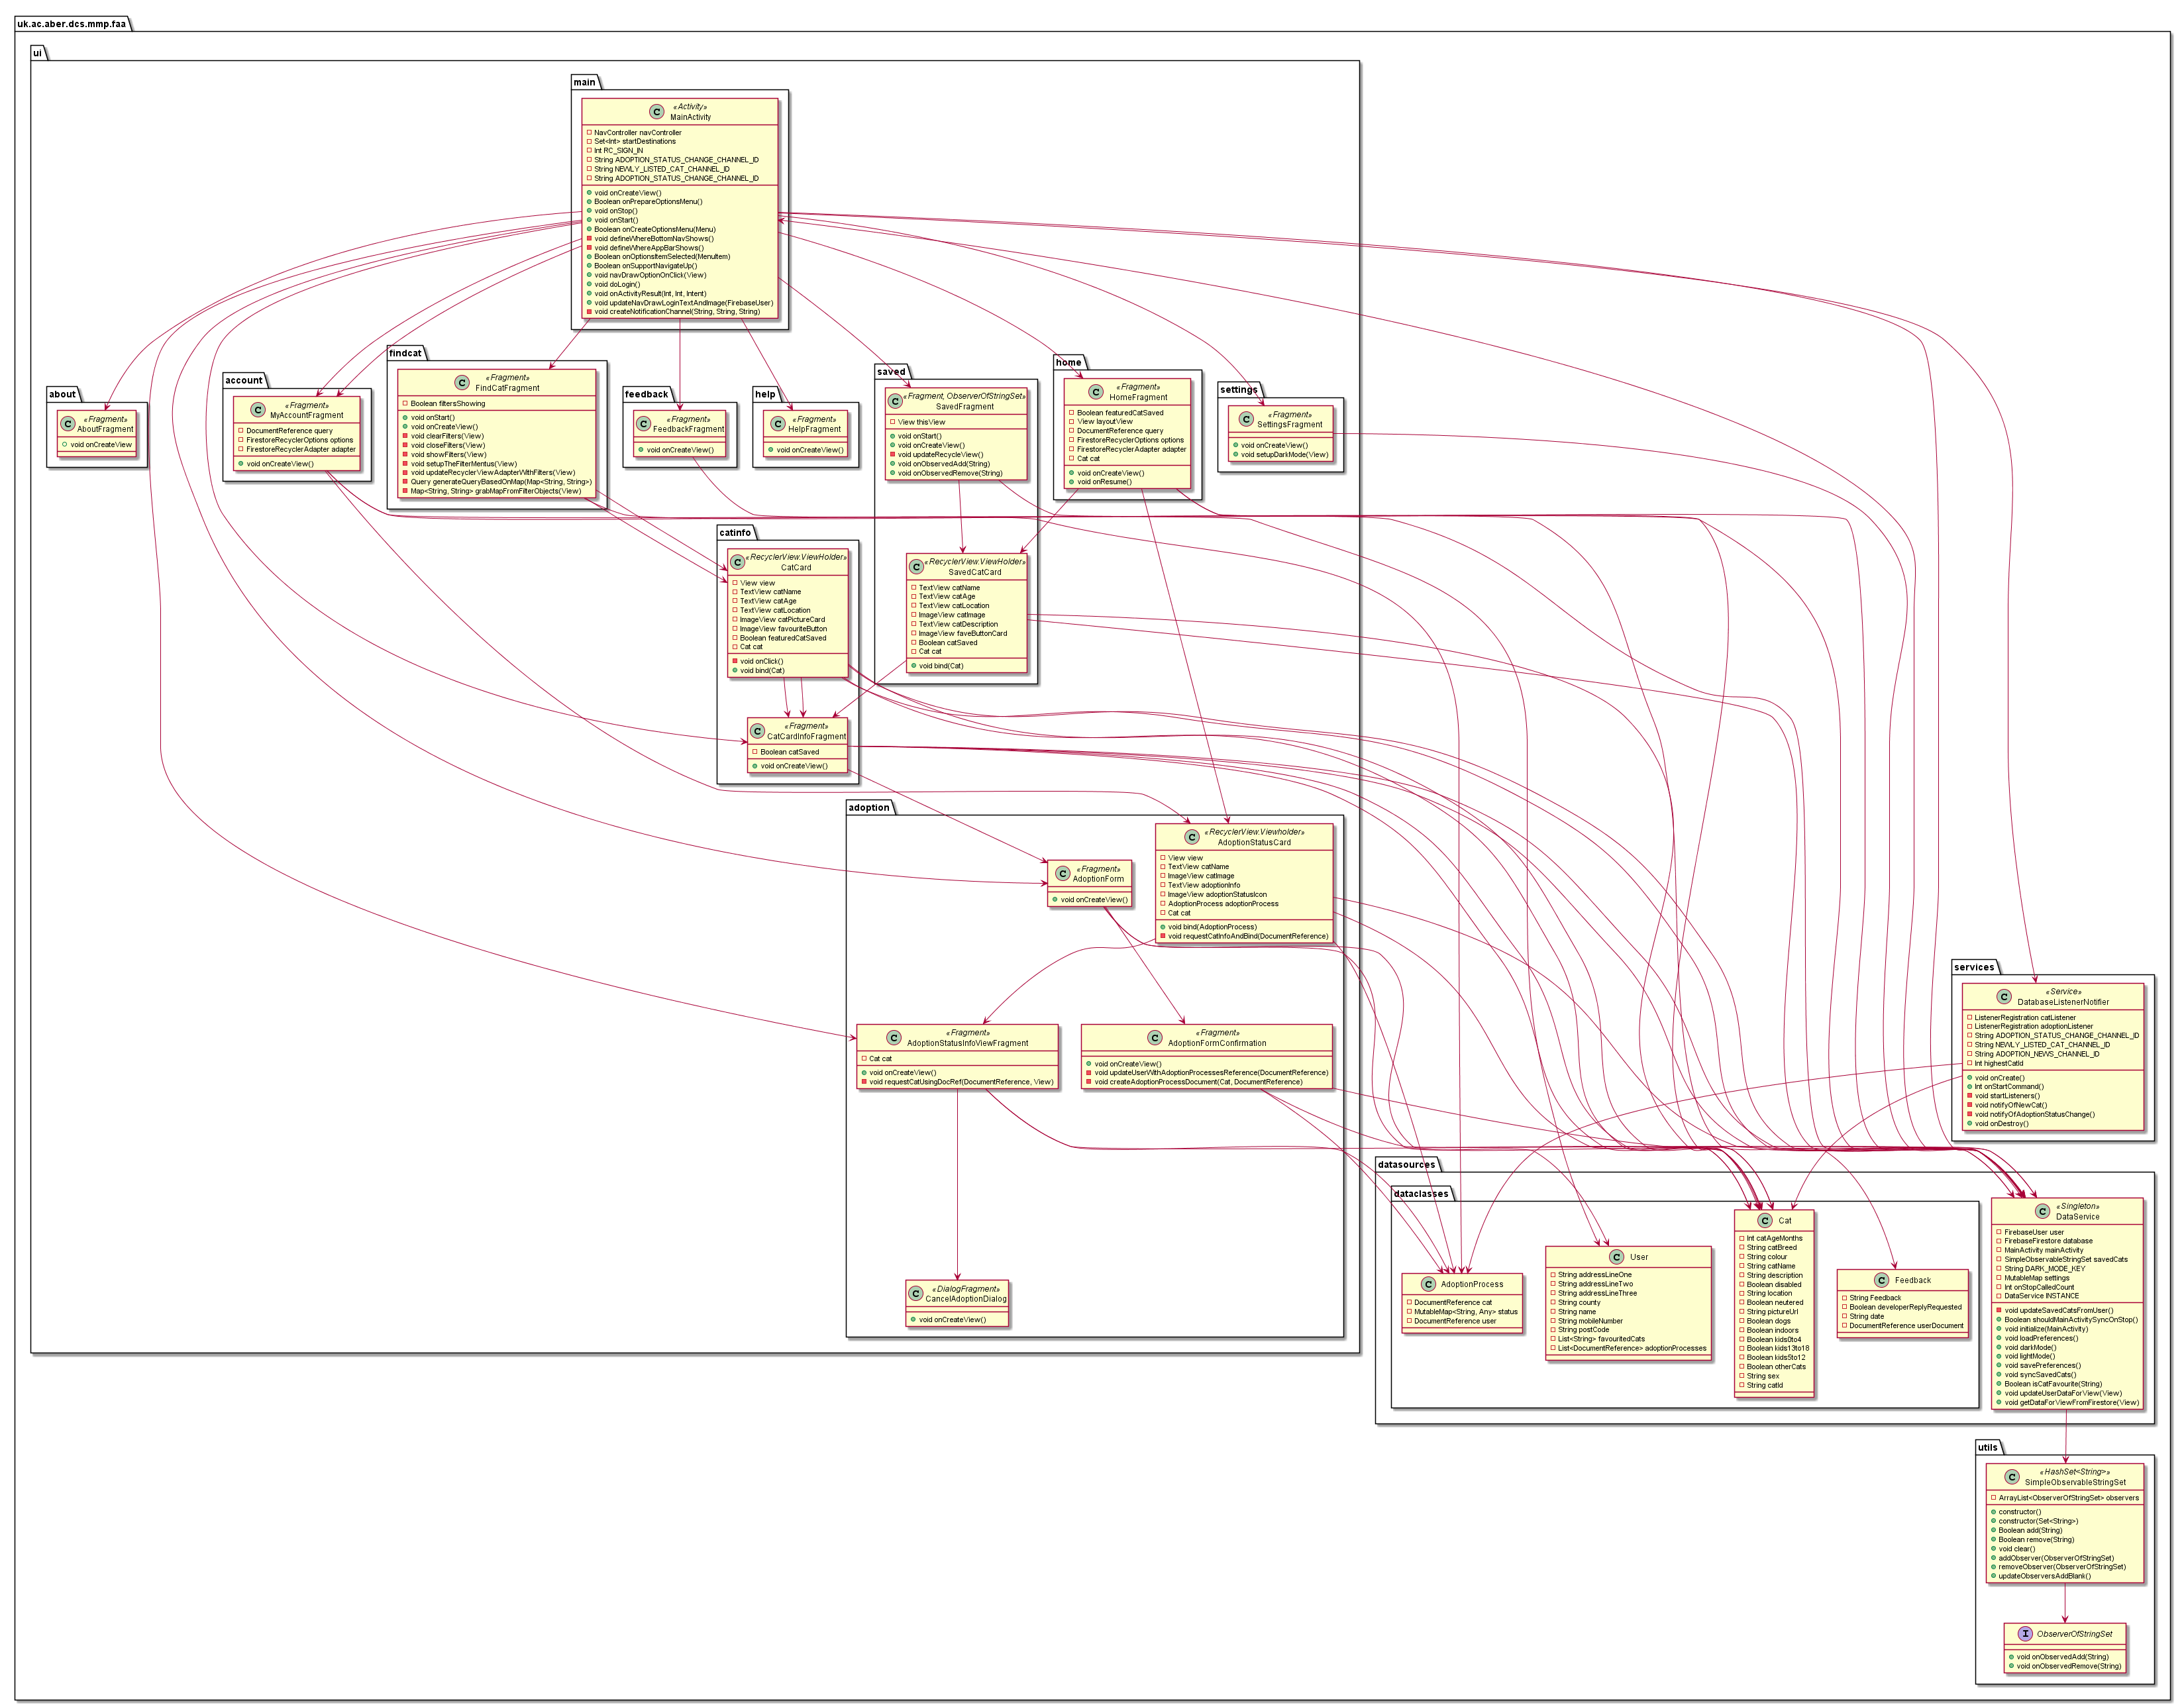
\includegraphics[scale=0.18]{Images/ClassDiagram.png}
            \caption{UML Class Diagram}
            \label{fig:classDiagram}
        \end{figure}
    \end{landscape}
    \subsection{Code structure}
    
    To show how the application's various classes fit together, I created the UML class diagram shown in Figure \ref{fig:classDiagram}. The application has various classes that all interact with each other, while classes are separated into packages ensuring more straightforward navigation in the project and separation of classes that have less in common with each other. To demonstrate the separation of packages look at the package under UI called adoption, it contains all UI elements that are concerned with the adoption process. 
    
    Many classes make use of the data classes which contain Cat, AdoptionProcess, User, and Feedback classes, where possible these classes are based on a Kotlin Data class, where it's explicit purpose is just for data storage, there is no particular need for these classes to do anything but that, it may be required however for some dataclasses to implement the Java Parcelable interface. Parcelable is required to transfer these data classes to the fragment that is being navigated to.

\subsection{DataService}

The DataService is a crucial part of the application, I have found through personal experience that using a central place for data retrieval throughout the application's UI elements allows me to cut down on spaghetti code and replace it with an interface that allows the UI to be interchangeable; This allows the data provider to be interchangeable, it's aim is to implement the role of the Presenter in a Model-View-Presenter relationship in GUI design \cite{MODELVIEWPRESENTER}. Due to the nature of the project, Google Firebase became a more vital interface and such in the project we have 2 DataServices, the local version for all data tracking not done with FirebaseFirebase, and the database reliant parts were done with the Firebase Firestore equivalent.

The DataService can be used by any of the parts of the application to call for a login request, and this is due to the nature of the DataService being initialised and owning a reference to the MainActivity, this is used throughout the application where being logged in is required to perform specific actions. The depth to which the DataService class is used is highlighted during the sequence of events that take place in the adoption process shown in the UML Sequence Diagram in Figure \ref{fig:sequenceDiagram}.

The DataService functionality is primarily inspired by the AnalysisDataService, which is an implementation of a DataService \cite{MANTIDDATASERVICE} class from the project I worked on during my Industrial Year, which held application-wide data for retrieval by individual interfaces.

        \begin{figure} [htbp!]
            \centering
            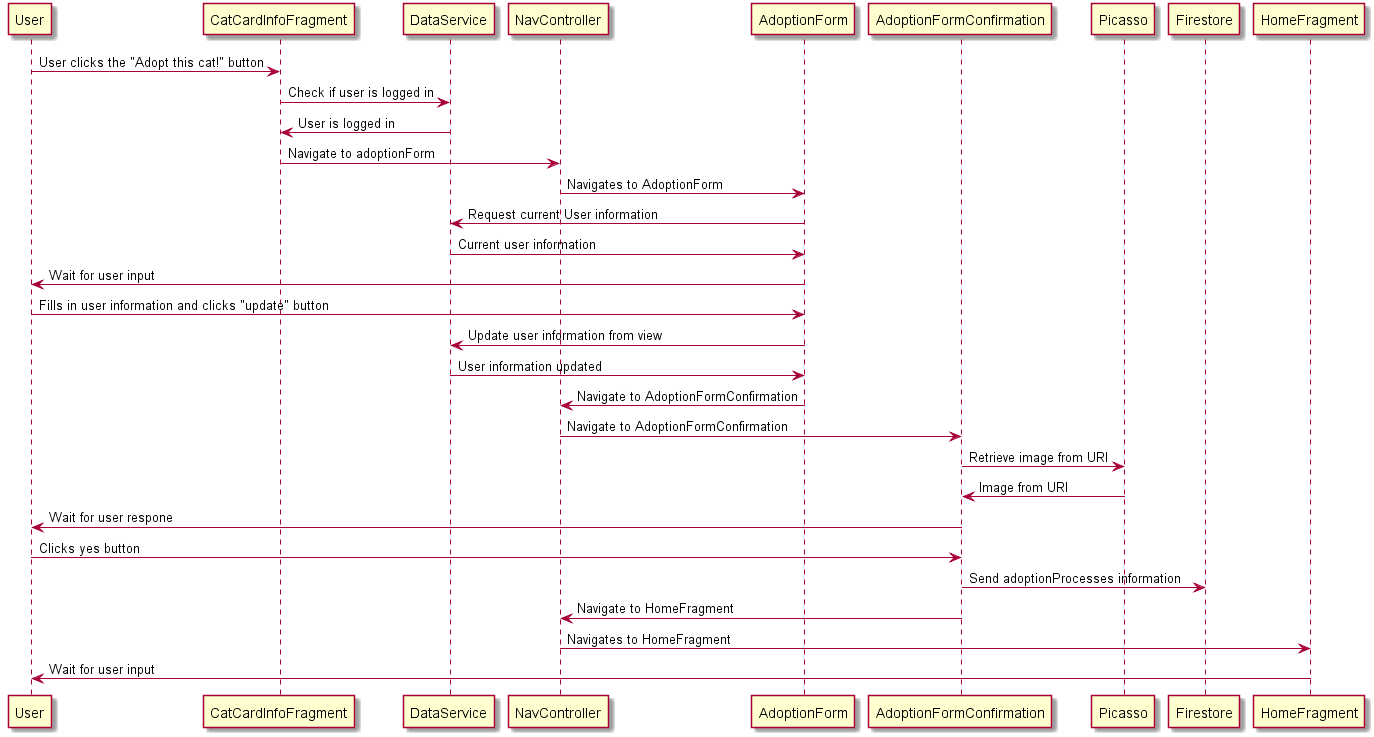
\includegraphics[width=\textwidth]{Images/Sequence Diagram Adoption Button Click.png}
            \caption{UML Sequence Diagram for adoption button being clicked}
            \label{fig:sequenceDiagram}
        \end{figure}
\subsection{MainActivity}

Due to the nature of a one Activity many fragment Android application, some significant functionality must be implemented in the aptly named MainActivity. The name is accurate as it is my only Activity. It is not the only Activity in the application, but the only one directly created by the project as Firebase Authentication runs in a separate activity. 

The MainActivity handles, the creation of the Navigation Draw, \gls{Bottom Navigation Bar} and it's configuration, Navigation Controller, Logging in, Notification Channel creation, and the application bar and its configuration. Parts of the MainActivity where it handles configuration is where these items are displayed, for example, the \gls{Bottom Navigation Bar} is only shown in main locations of the app, these are the HomeFragment, CatFinderFragment, and SavedCatFragments.

All Activity related Android lifecycle elements and primary setup and initialisation must occur in this one class, to stick to the One Activity, Many Fragments \cite{ONEACTIVITYMANYFRAGMENTS} methodology that is implemented in so many modern applications. 

Multiple activities require in some cases up to 2x CPU usage. On mobile devices, CPU is a limited resource and thus reducing CPU usage is key to a fast and smooth running device and application. The reason multiple activities require increased CPU usage is due to the nature of Activity creation and destruction on Android as data is regenerated un-necessarily when creating more Activities \cite{ONEACTIVITYMANYFRAGMENTS}. This decreased CPU usage is at the cost of a small increase to memory usage; almost all modern phones have enough memory for this not to be noticeable. With the added benefit for a developer having greater control over the application, with simple interfacing with the navigation controller using NavigationUI \cite{NAVIGATIONUI}, it is a superior method of Android application implementation.

\section{Accessibility} \label{ACCESSIBILITYDESIGN}
In the modern-day, it is increasingly hard to socially interact and perform specific tasks without a mobile device; this, however, is not accessible to a large portion of the population without particular adaptations. For example, if someone is unable to see the smaller text on a small device, they may use a tablet, having your interface increase in size to that of a table would allow a user to see things that they couldn't otherwise. In this section, a discussion takes place for the design decisions that have been taken to adhere to the accessibility of people to this application across need barriers. Android already has many accessibility features built-in, and there is a set of guidelines to follow to best assist in their functionality \cite{ACCESSIBILITYPRACTICES}.
    \subsection{Text Size}
    The size of text should scale to the size of the screen using it, and this doesn't inherently happen in Android applications. Historically developers would use point size to discern the size of the text in their layouts; however as Android has been updated, it has introduced scale-independent pixels which scale with the size of the screen a user is using, alongside layouts that are designed to do the same. It is planned to implement scale-independent pixels for all text in the application. It is currently not completed.

Android offers the ability however to enlarge all text across all applications inside of its accessibility settings, so this feature was pushed down the road, as it is possible without specific support to users who understand the features available in the settings.
    \subsection{Layout Scalability - Tablet Support}
    I have tested that the app works on a tablet, it is functional however it does not look as sleek as on a mobile phone for which this application was designed, but it is functional and combined with built-in Accessibility features in Android such as display scaling looks much sleeker. There is a plan to support this more extensively without the need to utilise Accessibility features built into Android as people may struggle to find those in the first place, however, the breadth of this implementation is time-limited.
    \subsection{Start to End support throughout}
    To support many locations across the globe, modern Android has implemented start to end layout opposed to left to right, and this provides support for people in areas that use right to left in literature as it may make it easier for users from these areas to more easily adopt Android. To support start to end layouts, all layouts in the application are created using Start to End implementation instead of left to right implementation. To increase user base and usability for users with a right to left layout, this accessibility is both easy to implement and vital.
    \subsection{Content Description for images}
    For people who are blind or hard of sight, it is important to provide a content description for all images, this is encouraged in Android Studio and is also simple to implement in multiple languages for internationalisation using strings. Content descriptions are read using computer-generated voices to users who are blind or hard of sight, much like the text is read, this is a feature baked into Android itself, but the application has added extra support for this in the form of the Content-Description for images.